\documentclass[9pt,shortpaper,twoside,web]{ieeecolor}
\usepackage{generic}
\usepackage{cite}
\usepackage{amsmath,amssymb,amsfonts}
\usepackage{algorithmic}
\usepackage{dsfont}
\usepackage{graphicx}
\usepackage{textcomp}
\usepackage{epsfig}
\usepackage{tikz}
\newcommand*\circled[1]{\tikz[baseline=(char.base)]{
            \node[shape=circle,draw,inner sep=2pt] (char) {#1};}}
\def\BibTeX{{\rm B\kern-.05em{\sc i\kern-.025em b}\kern-.08em
    T\kern-.1667em\lower.7ex\hbox{E}\kern-.125emX}}
\markboth{\journalname, VOL. XX, NO. XX, XXXX 2017}
{Author \MakeLowercase{\textit{et al.}}: Preparation of Brief Papers for IEEE TRANSACTIONS and JOURNALS (February 2017)}
\begin{document}
\title{Learning at the Racetrack: Data-driven Methods to Improve Racing Performance over Multiple Laps}
\author{Nitin R. Kapania and J Christian Gerdes
\thanks{This work was supported in part by the National Science Foundation Graduate Research Fellowship Program and the Stanford Graduate Fellowship. }
\thanks{Nitin Kapania is a postdoctoral fellow at Stanford University and a visiting scholar at UC Berkeley (e-mail: nkapania@stanford.edu).}
% \thanks{S. B. Author, Jr., was with Rice University, Houston, TX 77005 USA. He is 
% now with the Department of Physics, Colorado State University, Fort Collins, 
% CO 80523 USA (e-mail: author@lamar.colostate.edu).}
\thanks{J. C. Gerdes is a Professor 
at Stanford University (e-mail: gerdes@stanford.edu).}}

\maketitle

\begin{abstract}
Autonomous vehicles will generate data from the variety of sensors they employ to track the surrounding environment. This data is inherently valuable, as it gives algorithm designers the potential to leverage prior experience in order to improve driving performance over time. This paper uses the lens of autonomous racing to provide an example of how data from previous iterations of driving can be used to improve quantitative metrics of performance. Two complementary algorithms are demonstrated in this paper. The first algorithm uses iterative learning control (ILC) to simultaneously improve lateral and longitudinal tracking of the desired racing trajectory over multiple laps, while the second algorithm is focused on altering the trajectory itself using a search method. When driven experimentally at the limits of handling, the result is a reduction in lap time of nearly 1.4 seconds, a major improvement.    

\end{abstract}

\begin{IEEEkeywords}
 Autonomous driving, iterative learning control, A* search
\end{IEEEkeywords}

\section{Introduction}
\label{sec:introduction}

\subsection{Problem Description and Proposed Solution}
Several methods exist in the literature to generate autonomous racing trajectories 
(\cite{casanova},\cite{kelly},\cite{theodosis},\cite{kapaniadscc}), which typically comprise of a longitudinal speed profile $U_x(s)$ and a desired curvature profile $\kappa(s)$ as a function of distance along the track. These trajectories can then be tracked using one of several path following controllers, such as (\cite{mickcop},\cite{fricStudy},\cite{mickgeneral},\cite{shladover},\cite{nagai}). 

Using the trajectory generated by \cite{kapaniadscc} and the trajectory following controller presented by \cite{kapania}, the
authors generated a test run of an autonomous race vehicle (see Fig.\ref{fig:carpic}) at the limits of handling on the Thunderhill Raceway course in Willows, CA. %(Fig.~\ref{fig:carpic}(b)). 
The results are shown in Fig. \ref{fig:expErrors}.

\begin{figure}[h]
\centering
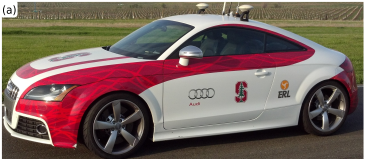
\includegraphics[width=2.5in]{figures/pic1.png}
\caption{``Shelley" - Stanford's autonomous self-driving race vehicle.}
\label{fig:carpic}
\end{figure}

\begin{figure}[h]
\centering
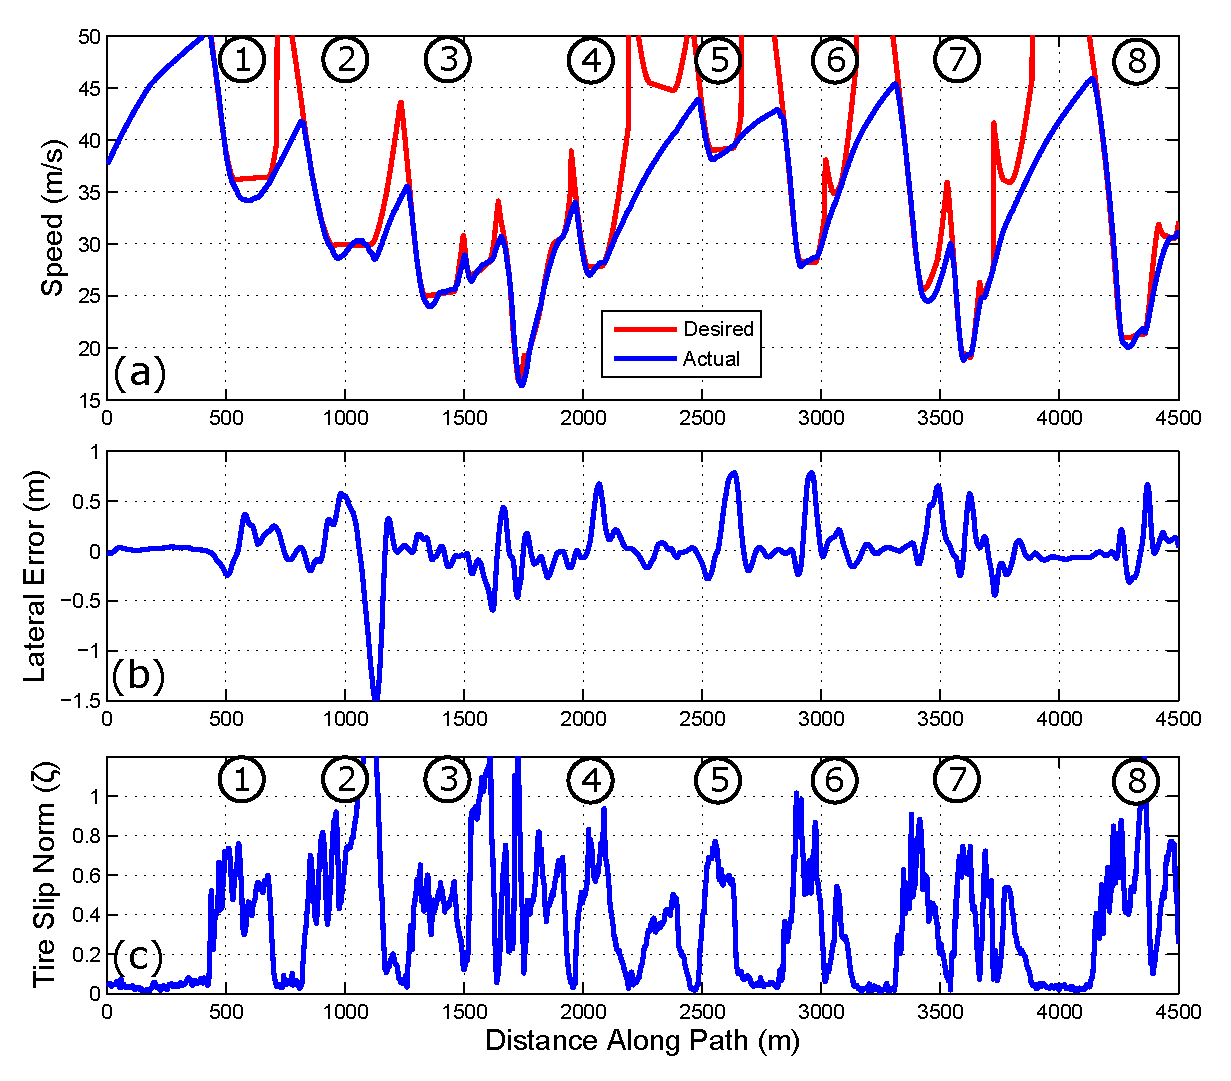
\includegraphics[width=2.8in]{figures/expErrors.eps}
\caption{Controller tracking performance and tire slip norm on a test run at the limits of handling ($\mu =$ 0.94).(a) Desired
vs actual speed of the vehicle. (b) Lateral tracking error and (c) tire slip norm as a function of distance along the path.}
\label{fig:expErrors}
\end{figure}

While the vehicle is able to generate lap times that are comparable to an amateur expert, the resulting lap times are 2-3 seconds below that of a professional human race car driver. There are several ways to analyze why this difference arises, but a simple insight that makes the case for lap-to-lap learning comes from viewing the trajectory tracking performance and friction utilization of the controller, shown in Fig.~\ref{fig:expErrors}. 

One of the issues shown in Fig.~\ref{fig:expErrors} is the relatively poor controller tracking on a few labeled sections of the race track. This includes errors in the lateral path tracking 
(sections \circled{2}, \circled{4} - \circled{7}) and failing to drive at the desired speed (sections \circled{1}, \circled{2}, \circled{7}), resulting directly in a loss 
of lap time. The speed and lateral path tracking will be improved in this paper with the addition of iterative learning control
(ILC) algorithms.

The second issue shown in Fig.~\ref{fig:expErrors} is the inconsistent usage of the tire friction capacity, as judged by the tire slip norm metric.
The tire slip norm, formalized in \cite{mickthesis}, is given by $\zeta$:

\begin{equation}
\label{eq:zeta}
\zeta = \sqrt{\left(\dfrac{\alpha}{\alpha_{p}}\right)^2 + \left(\dfrac{\sigma}{\sigma_p}\right)^2}
\end{equation}

Where $\sigma$ and $\alpha$ are the maximum longitudinal and lateral tire slips over all four tires, and $\sigma_p$ and $\alpha_p$ are empirically
determined \textit{peak slip} values resulting in maximum longitudinal and lateral tire force generation. As a result, $\zeta < 1 $ corresponds to the tires having excess force generation capacity, while $\zeta > 1$ corresponds to tire saturation. 

Fig.~\ref{fig:expErrors} shows inconsistent usage of tire friction across many turns. On some turns (sections \circled{2} and \circled{8}), the vehicle significantly exceeds the limits of handling, and the car's stability control systems kick in to regain control, slowing the car down in the process. On other turns (sections \circled{3}, \circled{5}, and \circled{7}),
the vehicle uses only a portion of the available tire force, indicating the vehicle can actually drive with higher acceleration on the next lap. Learning from prior runs to find the optimal acceleration (or $\mu$ parameter) for each part of the track will also be accomplished in this paper via an A* search algorithm. 

\subsection{Relation to Prior Work}
\subsubsection{Iterative Learning Control}

Iterative learning control (ILC) is based on the notion that the performance of a system that executes the \textit{same task} multiple times can be improved by learning from previous executions (trials, iterations, or in our case, laps of racing) \cite{bristow}.
On every iteration, a control signal is applied to a system in order to follow an ideal, unchanging ``reference trajectory". 
The tracking error for that iteration is recorded, and a learning algorithm is applied to improve the control signal and achieve
more accurate system performance on the next iteration. There are a variety of learning algorithms used, but most attempt to correct the tracking error by using a model of the system to determine the augmentation to apply to the prior control signal. This process is repeated until the reference tracking performance becomes satisfactory.

Because iterative learning control works best when learning to follow the same reference trajectory under nearly constant ambient conditions, the most common applications of ILC are in the field of automated manufacturing. Notable examples include CNC machining \cite{kimdi}, industrial robotics \cite{freeman}\cite{hladowski}, piezolectric stage positioning \cite{huang}, motor control \cite{mohammad}, and microdeposition \cite{hoelzle}. However, the rise of automated systems outside factory environments has led to important applications of ILC for ground and air robotics. Chen and Moore \cite{chen} proposed a simple iterative learning scheme to improve path-following of a ground vehicle with omni-directional wheels. Purwin and Andrea synthesized an iterative controller using least-squares methods to aggressively maneuver a quadrotor unmanned aerial vehicle (UAV) from one state to another \cite{purwin}. Sun et al. \cite{sun} proposed an iterative learning controller for speed regulation of high-speed trains. Other novel applications where ILC has been applied include Homogeneous Charge Compression Ignition (HCCI) \cite{slepicka2016iterative} and wing vibration suppression \cite{xu2015iterative}.  

\subsubsection{Trajectory Modification Algorithms}

Iterative learning control (ILC) algorithms can help an autonomous vehicle follow a desired trajectory more precisely over several laps of driving. However, ILC algorithms do not alter the desired trajectory itself, only the input signals that attempt to track the trajectory. In cases where the trajectory results in oversteer or understeer, a trajectory modification algorithm is necessary since the vehicle may already be saturating the tires, and applying additional actuator effort will not result in better tracking.


Some trajectory modification algorithms previously investigated in
the literature have focused on modifying the \textit{lateral} trajectory by altering the curvature profile as the vehicle understeers or oversteers. For example, Theodosis and Gerdes presented an algorithm to gradually widen the radius of a turn in response to a detected understeer \cite{paulthesis}. Klomp and Gordon also developed a strategy for recovering from
vehicle understeer by solving for an optimal emergency braking profile to minimize deviation from the desired path \cite{klomp} Brown et al.~\cite{brown2017safe} presented a model predictive control (MPC) approach that generally aimed to follow a planned vehicle trajectory at the limits. However, if the vehicle was at risk of understeering or oversteering, the MPC algorithm would deviate laterally from the planned trajectory in order to maintain stability of the vehicle without driving off the road. Another approach to trajectory modification is Learning Model Predictive Control (LMPC), developed by Rosolia et al. \cite{rosolia2017autonomous} for the purpose of autonomous racing. In LMPC, data from every lap of racing is used to build invariant sets and approximate the value function for the generally non-convex lap time minimization problem.   

\subsection{Order of Contributions}

Due to the repetitive nature of automotive racing, iterative learning control techniques are a promising method to gradually eliminate \textit{trajectory tracking} errors. This paper will first present adaptations of two established ILC methods  
(proportional-derivative and quadratically optimal) for use in the Audi TTS racing system.  The ILC algorithms will be designed for combined lateral and longitudinal control, as an extension of the lateral-only ILC first presented in \cite{kapaniaacc}

Second, this paper will address situations where the vehicle underperforms due to excessive oversteer or understeer. An A* search algorithm is presented
that iteratively modifies portions of the \textit{velocity} profile to be more conservative if a stability violation is encountered on a prior lap. The algorithm also modifies the velocity profile to be more aggressive if the tires are not being actuated at the limits. In this way, the algorithm is focused on learning the time-optimal friction profile $\mu^\star(s)$ by searching through datasets obtained over multiple laps. 

\section{Iterative Learning Control}

\subsection{Dynamic System Model}
\label{sec:ch4dsm}
The ILC algorithms we consider require a set of closed-loop system dynamics that are (a) stable to any disturbance input, and (b) expressible as an \textit{affine} discrete dynamical system. In our case, we have two subsystems: the steering controller and the longitudinal speed control. Stability of the steering controller
under lanekeeping feedback was shown in the linear case by \cite{rossetter2002} and in the saturated case by \cite{talvala}. Similar analyses can be considered to show the stability of a simple proportional speed-following controller.

The more difficult task is expressing the dynamics of the two subsystems using an affine model, given the tendency for the vehicle tires to saturate at the limits. This paper will model the dynamics with a bicycle model with single longitudinal input $F_x$ and front steer input $\delta$, shown in Fig.~\ref{fig:bikemodel}.

\begin{figure}[h]
\centering
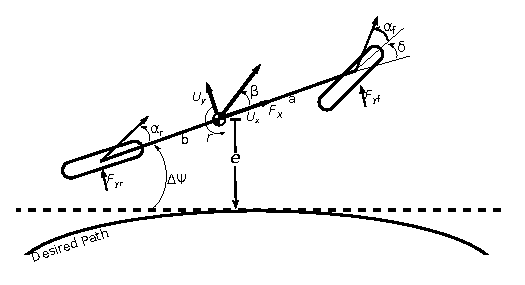
\includegraphics[width=3.5in]{figures/BikeModelSchematic.eps}
\caption{Schematic of bicycle model with steer input $\delta$ and longitudinal input $F_x$.}
\label{fig:bikemodel}
\end{figure}


% Nonlinear, coupled equations of motion are provided in (\ref{eq:fullNL})-(\ref{eq:fullNL2}):

% \begin{align}
% \label{eq:fullNL}
% 	\dfrac{de}{dt} &= \left(v+U^\mathrm{des}_x(s)\right)(\beta + \Delta\Psi) \\
% 	\dfrac{dv}{dt} &= \left(v+U^\mathrm{des}_x(s)\right)\beta r + \frac{F_x}{m} - \frac{F_\mathrm{yf}(\alpha_\mathrm{f},F_x)\delta}{m}\\
% 	\dfrac{d\beta}{dt} &= \frac{F_\mathrm{yf}(\alpha_\mathrm{f}, F_x) + F_\mathrm{yr}(\alpha_\mathrm{r},F_x)}{m\left(v + U^\mathrm{des}_x(s)\right)}-r \\
% 	\dfrac{dr}{dt}     &= \frac{aF_\mathrm{yf}(\alpha_\mathrm{f}, F_x) - bF_\mathrm{yr}(\alpha_\mathrm{r}, F_x)}{I_z} \\
% 	\dfrac{d\Delta\Psi}{dt} &= r - \kappa(s)(v+U^\mathrm{des}_x(s)) \label{eq:fullNL2}
% \end{align}
% The system dynamics presented in (\ref{eq:fullNL}) have five states, yaw rate $r$, vehicle sideslip $\beta$, lateral path tracking error $e$, heading error $\Delta \Psi$, and speed tracking error $v$, defined by:

% \begin{equation}
% v = U_x - U^\mathrm{des}_x
% \end{equation}

The potential for coupling between the subsystems occurs from both the state equations and also the complex nature of tire force generation at the handling limits. As shown in Fig.~\ref{fig:coupledTires}, as longitudinal force $F_x$ is distributed across the tires, the available lateral force decreases. At the limits of handling, this \textit{derating} of the lateral force may become significant. As a result, we model lateral tire force generation $F_y$ as a function of both lateral tire slip $\alpha$ and the applied longitudinal force $F_x$, using a modified form of the Fiala tire model \cite{rami}. 
\begin{figure}[tb]
\centering
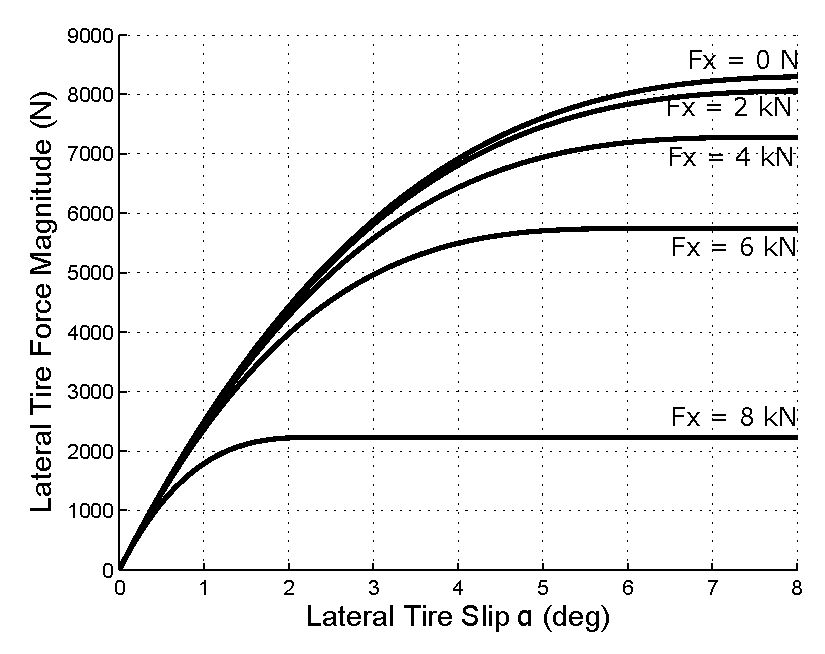
\includegraphics[width=2.8in]{figures/tirecurves.eps}
\caption{Lateral tire force curve as a function of longitudinal force $F_x$ and lateral tire slip $\alpha$.}
\label{fig:coupledTires}
\end{figure} 

The control inputs $F_x$ and $\delta$ are broken up into the closed-loop feedback term and the \textit{learned} component that is modified on every lap by the ILC algorithm:
\begin{align}
\label{eqn:splitTerms}
F_x &= F^{\mathrm{FB}}_x + F^L_x\\
    &= -K_xv + F^L_x\\
\delta &= \delta_{\mathrm{FB}} + \delta_L\\
\delta &= -k_p(e + x_\mathrm{LA}\Delta\Psi) + \delta_L
\end{align}
where $K_x$ is the proportional speed tracking gain and $k_p$ and $x_\mathrm{LA}$ are the lookahead gains presented in \cite{kapania}. The term $v$ denotes the speed tracking error.

The closed loop system dynamics are given by incorporating (\ref{eqn:splitTerms}) into equations of motion for the bicycle model: 
\begin{align}
\label{eq:fullNLCL}	
	\frac{de}{dt} &= \left(v+U^\mathrm{des}_x(s)\right)(\beta + \Delta\Psi) \\
	\frac{dv}{dt} &= \left(v+U^\mathrm{des}_x(s)\right)\beta r + \frac{-K_xv + F^L_x}{m} \\
	& - \frac{F_\mathrm{yf}(\alpha_F,F_x)(k_p(e + x_{LA}\Delta\Psi) + \delta_L)}{m}\\
	\frac{d\beta}{dt} &= \frac{F_\mathrm{yf}(\alpha_\mathrm{f}, F_x) + F_\mathrm{yr}(\alpha_\mathrm{r},F_x)}{m\left(v + U^\mathrm{des}_x(s)\right)} - r \\
	\frac{dr}{dt}     &= \frac{aF_\mathrm{yf}(\alpha_\mathrm{f}, F_x) - bF_\mathrm{yr}(\alpha_\mathrm{r}, F_x)}{I_z} \\
	\frac{d\Delta\Psi}{dt} &= r - \kappa(s)(v+U^\mathrm{des}_x(s))\label{eq:fullNLCL2}	
\end{align}

The nonlinear closed-loop dynamics must be converted into an affine, discrete-time dynamical system to apply conventional iterative learning
control algorithms. In our case, we have two system outputs ($y = [e \hspace{2mm} v]^T$) that are measured and two input signals to learn ($u = [\delta_L \hspace{2mm} F^L_x]^T$). 
Since we run the iterative learning control algorithm after seeing a trial of data, we can approximate
the dynamics in (\ref{eq:fullNLCL})-(\ref{eq:fullNLCL2}) by linearizing about the observed states and inputs $x_o, u_o$ from the first lap. These state estimates can be obtained from a differential GPS, simulation, or a state observer. The affine model is therefore given by: 
 \begin{align}
 \label{eq:ssMAT}
 \begin{bmatrix} \dot{e} \\ \dot{\beta} \\ \dot{r} \\ \dot{\Delta\Psi} \\ \dot{v}\end{bmatrix} &= \begin{bmatrix} A(t) \end{bmatrix} \begin{bmatrix} e \\ \beta \\ r \\ \Delta\Psi \\ v \end{bmatrix} + \begin{bmatrix} B(t) \end{bmatrix} \begin{bmatrix} \delta_L \\ F^L_x \end{bmatrix} + d(t) \\
 \begin{bmatrix} e \\ v \end{bmatrix}  &= \begin{bmatrix} 1 & 0 & 0 & 0 & 0 \\ 0 & 0 & 0 & 0 & 1 \end{bmatrix} x
 \end{align}
 
 The time-varying state space matrices $A(t)$ and $B(t)$ are given by Jacobian linearizations of the closed loop nonlinear dynamics (\ref{eq:fullNLCL}) about the observed states and inputs $x_o(t), u_o(t)$ from the last trial:
 \begin{align}
 \label{eq:C4nl}
 \begin{bmatrix} A(t) \end{bmatrix} &= \frac{\partial{f}}{\partial{x}}\Big|_{x_o(t)} \\
 \begin{bmatrix} B(t) \end{bmatrix} &= \frac{\partial{f}}{\partial{u}}\Big|_{u_o(t)}
 \end{align}

 This multiple-input, multiple-output (MIMO) model captures the coupled behavior of the longitudinal and lateral inputs. If we make the assumption that the longitudinal and lateral inputs are decoupled and make small angle approximations, we may obtain the following resulting analytical state matrices $A(t)$ and $B(t)$ for (\ref{eq:ssMAT}):

\begin{align}
\label{eqn:C4dyn}
 &A(t)  = \\ \nonumber
  &\left[\begin{smallmatrix}
  0 & U_x(t) & 0 & U_x(t) & 0\\ 
  0 & 0 & 1 & 0 & 0 \\ 
  \frac{-ak_\mathrm{p} \tilde{C}_\mathrm{f}(t)}{I_\mathrm{z}}  & \frac{-ak_\mathrm{p}x_\mathrm{LA}\tilde{C}_\mathrm{f}(t)}{I_\mathrm{z}}  & \frac{-a^2\tilde{C}_\mathrm{f}(t)-b^2\tilde{C}_\mathrm{r}(t)}{U_x(t)I_\mathrm{z}} & \frac{b\tilde{C}_\mathrm{r}(t) - a\tilde{C}_\mathrm{f}(t)}{I_\mathrm{z}} & 0 \\
  \frac{-k_\mathrm{p}\tilde{C}_\mathrm{f}(t)}{mU_x(t)}  & \frac{-k_\mathrm{p}x_\mathrm{LA}\tilde{C}_\mathrm{f}(t)}{mU_x(t)}  & \frac{b\tilde{C}_\mathrm{r}(t)-a\tilde{C}_\mathrm{f}(t)}{mU_x(t)^2}-1 & \frac{-\tilde{C}_\mathrm{f}(t) - \tilde{C}_\mathrm{r}(t)}{mU_x(t)} & 0 \\
  0 & 0 & 0 & 0 & -\frac{K_x}{m}
  \end{smallmatrix}\right] \\
&B(t) =\begin{bmatrix} 0 & 0 \\	 	0 & 0 		\\ 		\frac{a \tilde{C}_\mathrm{f}(t)}{I_\mathrm{z}} & 0 		\\ 		\frac{\tilde{C}_\mathrm{f}(t)}{mU_x(t)} & 0 		\\ 0 & \frac{1}{m} \end{bmatrix} 
\end{align}
The affine term $d(t)$ is given by: 
\begin{align}
d(t) = \left[\begin{matrix} 0 \\
               -\kappa(t) U_x(t) \\ 
			    \frac{a\tilde{C}_\mathrm{f}(t)\tilde{\alpha}_\mathrm{f}(t) - b\tilde{C}_\mathrm{r}(t)\tilde{\alpha}_\mathrm{r}(t) + a\tilde{F}_\mathrm{yf}(t) - b\tilde{F}_\mathrm{yr}(t)}{I_z}\\
				\frac{\tilde{C}_\mathrm{f}(t)\tilde{\alpha}_\mathrm{f}(t) + \tilde{C}_\mathrm{r}(t)\tilde{\alpha}_\mathrm{r}(t) + \tilde{F}_\mathrm{yf}(t) + \tilde{F}_\mathrm{yr}(t)}{mU_x(t)}\\
				0 \\
				0
				\end{matrix}\right]
\end{align}


Where $\tilde{F}_\mathrm{yf,r}(t)$ are the steady-state front and rear tire forces from the first lap, $\tilde{C}_\mathrm{f,r}(t)$ are the effective cornering stiffnesses at those tire forces, and $\tilde{\alpha}_\mathrm{f,r}(t)$ are the corresponding front and rear tire slips. While (\ref{eqn:C4dyn}) is written as a MIMO system for compactness, assuming decoupled lateral and longitudinal 
dynamics provides two single-input, single-output (SISO) systems. 

While beyond the scope of this paper, it should also be noted that advances in ILC research have focused specifically on ILC for nonlinear \cite{xunonlinear} and linear parameter-varying (LPV) systems \cite{de2017iterative}. 

\subsection{Lifted Domain Representation and ILC \newline Problem Statement}
\label{sec:liftedD}
Whether the coupled (\ref{eq:C4nl}) or decoupled (\ref{eqn:C4dyn}) dynamics are assumed, the
final modeling step is to apply the matrix exponential discretization technique to obtain dynamics in the following form:
\begin{align}
\label{C4ad}
x_{k+1} &= A_kx_k + B_ku_k + d_k \\
y_{k}   &= Cx_k
\end{align}
For a given lap of racing $j$, sensor measurements provide $N$ observations of both the lateral path deviation $e$ and longitudinal
speed tracking error $v$. These measurements can be stacked into a 2$N \times 1$ array: 
\begin{equation}
\mathbf{e}_j = \begin{bmatrix} e_1 & \hdots & e_N & v_1 & \hdots & v_N \end{bmatrix}^T
\end{equation} 
These measurement errors are related to the learned control inputs $\delta^L$ and $F^L_x$ as follows: 
\begin{align}
\label{eq:liftedDomain}
\mathbf{e}_j &= P\mathbf{u}^L_j + \mathbf{w} \\
\mathbf{u}^L_j &= \begin{bmatrix} \delta^L_1 & \hdots & \delta^L_N & F^L_{x1} & \hdots & F^L_{xN} \end{bmatrix}^T
\end{align}
The system dynamics modeled in the previous section are represented by the \textit{lifted-domain} dynamics matrix $P$,
which is $\mathrm{2}N \times \mathrm{2}N$ and given by:
\begin{equation}
\label{eq:C4bm}
P=\left[
\begin{array}{c|c}
P_{e\delta} & P_{eF} \\ \hline
P_{v\delta} & P_{vF} 
\end{array}\right]
\end{equation}
Where each submatrix in (\ref{eq:C4bm}) is $N \times N$ and represents the lifted-domain dynamics from a given input to a given output. 
Individual terms of the sub-matrices are given by:

\begin{equation}
\label{eq:how2Lift}
p_{lk} = \begin{cases} 0 &\mbox{if } l < k \\ 
C_yB_u(k) & \mbox{if } l = k \\
C_yA(l)A(l-1)\cdots A(k)B_u(k) &\mbox{if } l > k \end{cases}
\end{equation} 
Where $C_y$ is the row of $C$ in (\ref{C4ad}) corresponding to the desired output and $B_u$ the column of $B$ in (\ref{C4ad})
corresponding to the desired input. The term $\mathbf{w}$ in (\ref{eq:liftedDomain}) is the unknown disturbance. Iterative
learning control relies on the assumption that this disturbance is the underlying cause of the observed errors $\mathbf{e}_j$, and that the disturbance, while unknown, is constant from lap to lap.

Given the error signal $\mathbf{e}_j$ for a given lap $j$, the iterative learning problem is to find the inputs $\mathbf{u}_{j+1}$ that will cancel out the tracking error on the next lap. The learned inputs are then applied, the observed error $\mathbf{e}_{j+1}$ is recorded,
and the process is repeated until the tracking error falls to a desired level. There is a wide body of literature on methods to determine $\mathbf{u}_{j+1}$ given $P$ and $\mathbf{e}_j$, but this paper will compute the ILC input for the next lap with the following formulation:

\begin{align}
 \label{eqn:ctrlLaw}
 \mathbf{u}^L_{j\!+\!1} = Q(\mathbf{u}^L_j - L\mathbf{e}_j)
\end{align}
where $Q$ is the $2N \times 2N$ \textit{filter} matrix, and $L$ is the $2N \times 2N$ \textit{learning} matrix. 
In the following two sections, the
matrices $Q$ and $L$ will be obtained by designing a proportional-derivative (PD) iterative learning controller as well as a quadratically
optimal (Q-ILC) learning controller.

\subsection{Proportional-Derivative Controller}
\label{sec:pdcontroller}

The proportional-derivative ILC computes the steering $\delta^L$ and force $F^L$ correction for the current lap $j$ based on the error and 
error derivative at the same time index $k$ from the previous lap:
\begin{align}
	\label{eq:PDlaw}
	\delta^L_{j}(k) &= \delta^L_{j\!-\!1}(k) - k_{p\delta}e_{j\!-\!1}(k) - k_{d\delta}(e_{j\!-\!1}(k) - e_{j\!-\!1}(k-1))\\
	    F^L_{j}(k) &=  F^L_{j-1}(k) - k_{pF}v_{j\!-\!1}(k) - k_{dF}(v_{j\!-\!1}(k) - v_{j\!-\!1}(k-1))
\end{align}
where $k_{p\delta}$ and $k_{pF}$ are proportional gains and $k_{d\delta}$ and $k_{dF}$ are derivative gains. 
 
 The PD equation (\ref{eq:PDlaw}) determines $\delta^L$ only using lateral path deviation $e$ and $F^L_x$ using only the speed tracking error $v$. The filter matrix $Q$ is obtained by taking any filter transfer function and converting into the lifted domain via (\ref{eq:how2Lift}).  An important design consideration in choosing the two $k_p$ and $k_d$ gains is avoiding a poor lap-to-lap ``transient" response, where the path tracking error increases rapidly over the first several laps before
eventually decreasing to a converged error response $e_\infty$. This is a commonly encountered design requirement
for ILC systems, and can be solved by ensuring the following \textit{monotonic convergence} condition is met \cite{bristow}:

\begin{equation}
	\gamma \triangleq \bar{\sigma}(PQ(I-LP)P^{-1}) < 1
	\label{eq:MS}
\end{equation}
where $\bar{\sigma}$ is the maximum singular value. In this case, the value of $\gamma$ provides an upper bound on the change
 in the tracking error norm from lap to lap, i.e. 
 
\begin{equation}
	||\mathbf{e}_\infty - \mathbf{e}_{j+1}||_2 \leq \gamma ||\mathbf{e}_\infty-\mathbf{e}_j||_2
\end{equation}

Fig.~\ref{fig:stabPlot} shows values of $\gamma$ for both an unfiltered PD controller ($Q = I$), and for a PD controller with a 2 Hz, first order low pass filter. The $\gamma$ values are plotted as a
contour map against the controller gains $k_{p\delta}$ and $k_{d\delta}$. Addition of the low-pass filter
assists with monotonic stability by removing oscillations in the control input generated when trying to remove small reference tracking errors after several iterations.
The plot shown in Fig.~\ref{fig:stabPlot} is for the steering ILC design only, but the same analysis is possible for the longitudinal
ILC design as well. Because the $P$ matrix in general can change from iteration to iteration and will also
 change depending on the trajectory, making a general assertion or proof about stability of the iterative learning controller is difficult. 

\begin{figure}[tb]
\centering
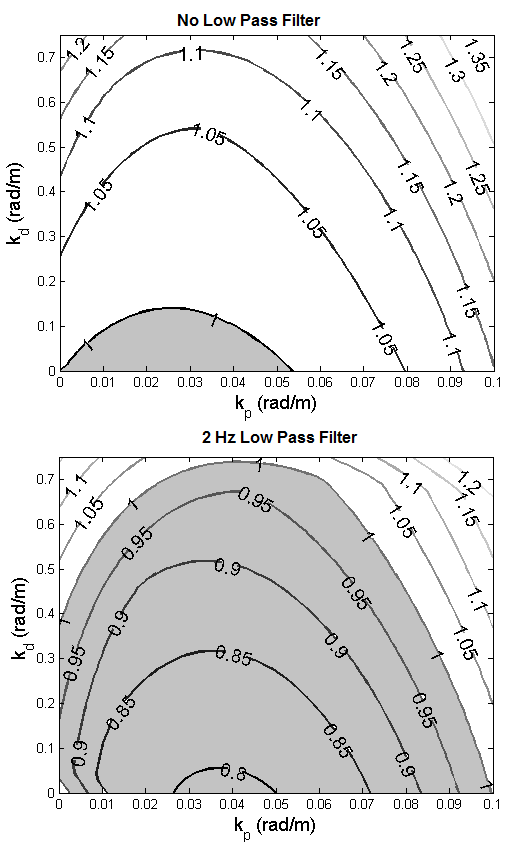
\includegraphics[width=2 in]{figures/monotonicStability.png}
\caption[Values of convergence bound $\gamma$ vs. $k_{p\delta}$ and $k_{d\delta}$ for PD iterative learning controller]{Values of convergence bound $\gamma$ vs. $k_{p\delta}$ and $k_{d\delta}$ for PD iterative learning controller with (top) no filtering and (bottom) with a 2 Hz low-pass filter. Lower values of $\gamma$ correspond to faster convergence.
Shaded regions correspond to gains that result in system monotonic stability. The stability analysis in Fig.~\ref{fig:stabPlot} assumes the $P$ matrix is constant for all iterations and is generated assuming decoupled vehicle dynamics
 for a straight-line trajectory at a constant speed of 20 m/s.}
\label{fig:stabPlot}
\end{figure}


\subsection{Quadratically Optimal Controller}\label{sec:controller}
\label{sec:qopt}
An alternate approach to determining the learned steering and longitudinal force input is to minimize a quadratic cost function for the next lap:

\begin{align}
J_{j\!+\!1} = \textbf{e}_{j\!+\!1}^TT\textbf{e}_{j\!+\!1} + \textbf{u}^T_{j\!+\!1} R \textbf{u}^T_{j\!+\!1}+\Delta_{j\!+\!1}^TS\Delta_{j\!+\!1}
\label{eq:QILC}
\end{align}
where $\Delta_{j\!+\!1} = \mathbf{u}^L_{j\!+\!1} - \mathbf{u}^L_j$ and the $2N \times 2N$ matrices $T$, $R$, and $S$ are weighting matrices, each given
by a scalar multiplied by the identity matrix for simplicity.
This formulation allows the control designer to weight the competing objectives of minimizing the tracking errors $e$ and $v$, control effort $|\delta^L|$ and $|F^L_x|$, and change in the control signal from lap to lap.
While constraints can be added to the optimization problem, the unconstrained problem in (\ref{eq:QILC}) can be solved analytically \cite{bristow2008} to obtain desired controller and filter matrices:

\begin{subequations}
\label{eq:analSol}
\begin{align}
	Q &= (P^TTP + R + S)^{-1}(P^TTP + S)\\
	L &= (P^TTP + S)^{-1}P^TTP(T^{1/2}P)^{-1}T^{1/2}
\end{align}
\end{subequations}

An advantage of the quadratically optimal control design over the simple PD controller is that the controller matrices $Q$ and $L$ take the linearized, time-varying dynamics $P$ into account. 
This allows the iterative learning algorithm
to take into account changes in the steering dynamics due to changes in vehicle velocity.
Furthermore, if the fully coupled dynamics (\ref{eq:C4nl}) are used, the iterative learning algorithm also accounts for the
second-order effect of steering on the longitudinal dynamics and longitudinal force application on the lateral dynamics. 
 However, a disadvantage is that computing $\mathbf{\delta}^L$ in (\ref{eqn:ctrlLaw}) requires matrix multiplications with
the typically dense matrices $Q$ and $L$ for every lap, which can be computationally expensive for fast sampling rates. 

\subsection{Simulated Results}
\label{sec:simres}

To test the feasibility of the PD and Q-ILC learning algorithms, the vehicle tracking performance over multiple laps is
simulated using the path curvature and speed profiles shown in Fig.~\ref{fig:simSetup}.
\begin{figure}[bh]
\centering
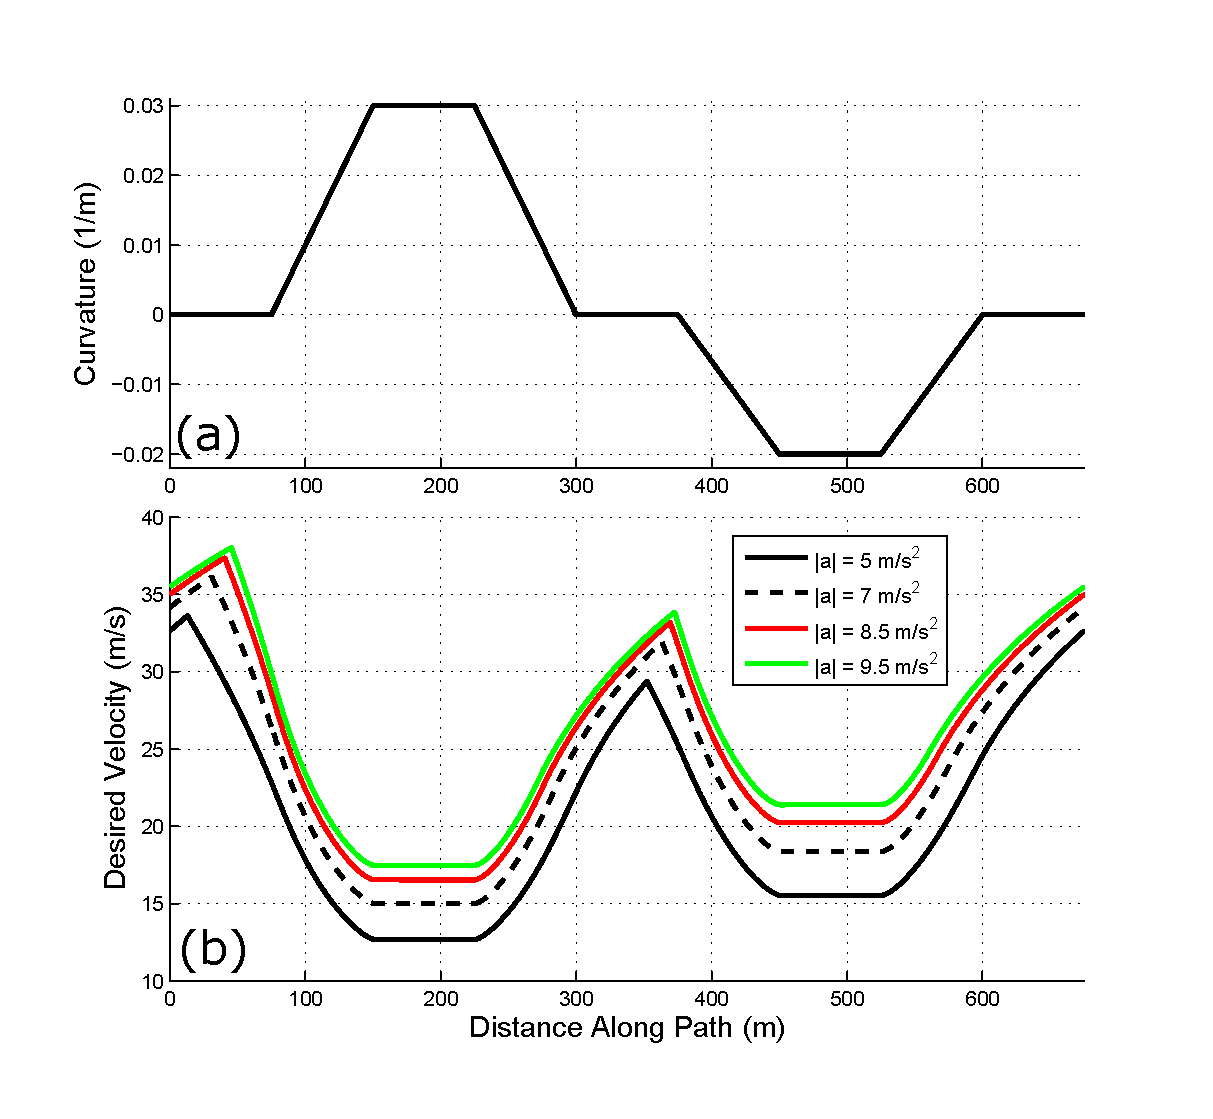
\includegraphics[width= 2.7in]{figures/simSetup.eps}
\caption[Curvature profile used for ILC simulation.]{ (a) Curvature profile used for ILC simulation. (b) Velocity profiles generated for four different levels of longitudinal/lateral acceleration. }
\label{fig:simSetup}
\end{figure}

Simulated results for the root-mean-square (RMS) lateral path deviation is shown in Fig.~\ref{fig:simRes1}. The results
show the change in RMS error as the number of ILC iterations increase. Three different ILC controllers are tested. 
The first controller is the simple PD controller
with low-pass filter (\ref{eq:PDlaw}), and the second controller is the quadratically optimal ILC algorithm (\ref{eq:analSol}) assuming fully coupled dynamics (\ref{eq:C4nl}) in the plant
matrix $P$ (i.e. the full MIMO system).
The third controller is also the quadratically optimal ILC algorithm, but the $P$ matrix used in the optimization
assumes decoupled dynamics (\ref{eqn:C4dyn}) and therefore solves the lateral and longitudinal SISO problems separately. 

\begin{figure}[h!]
\centering
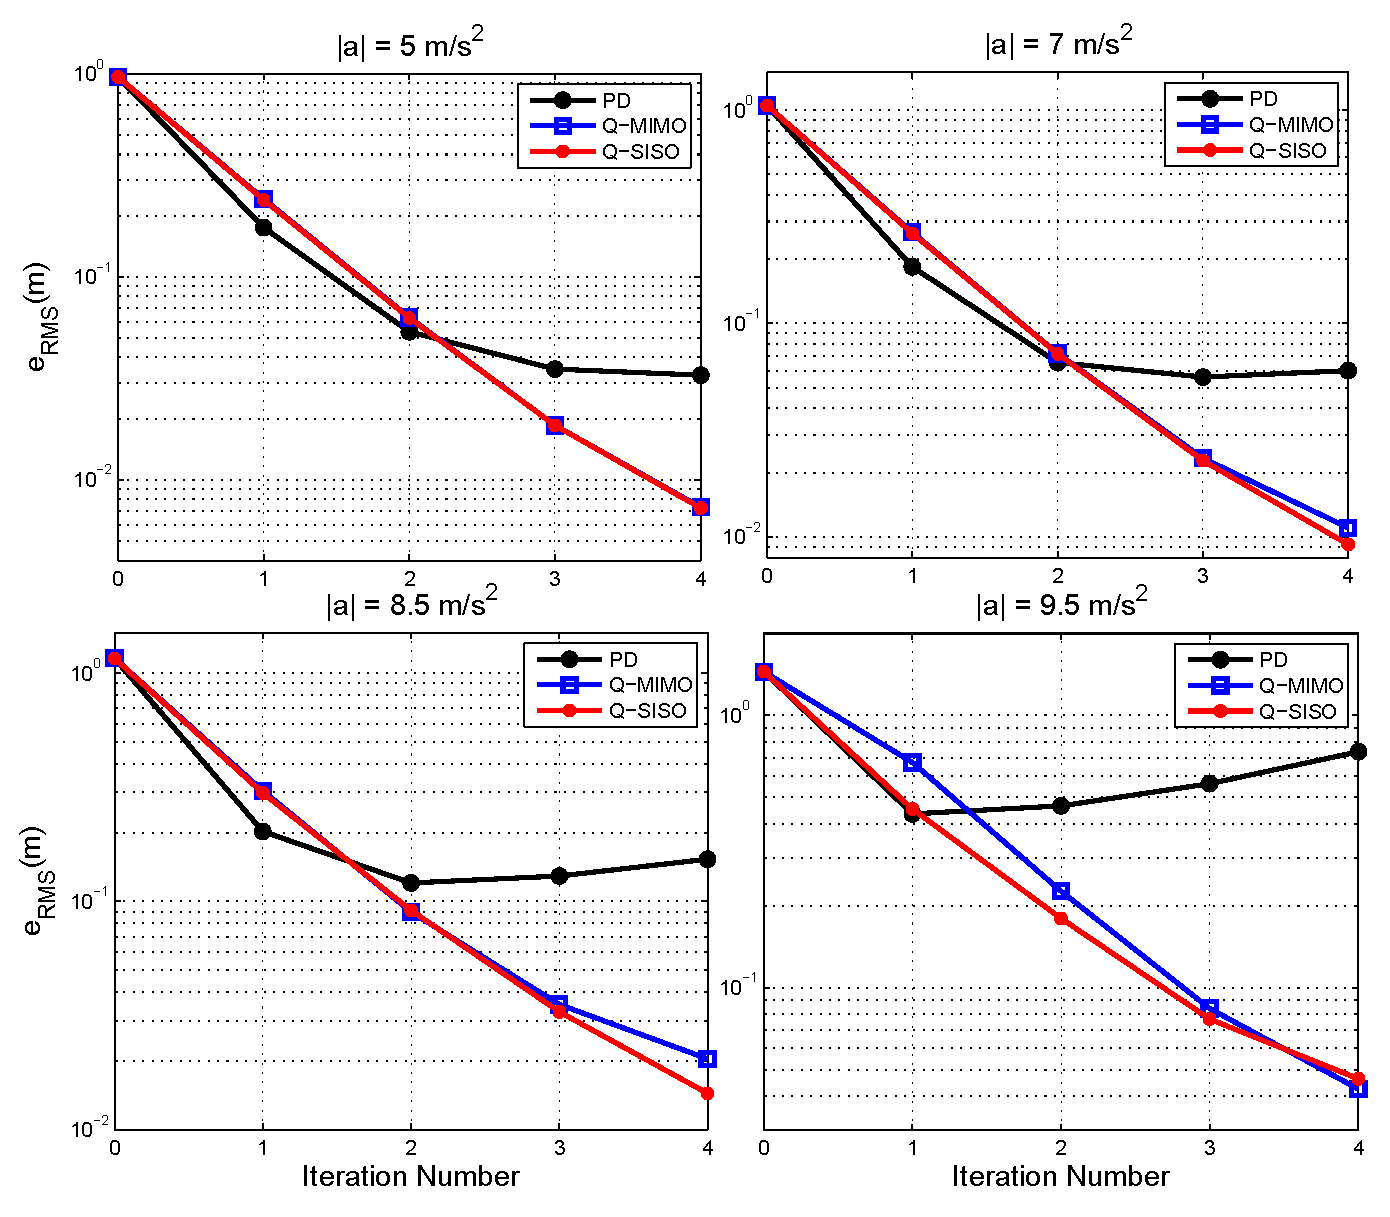
\includegraphics[width=3.5in]{figures/simRes1.eps}
\caption[Simulated results for root-mean-square path tracking error at several values of vehicle acceleration]{Simulated results for root-mean-square path tracking error at several values of vehicle acceleration, with $T = R = I$ and $S = \mathrm{100} I$.
Results are plotted on a log scale.}
\label{fig:simRes1}
\end{figure}

Fig.~\ref{fig:simRes1} shows that both quadratically optimal ILC algorithms exponentially reduce the lateral
path tracking error as the number of learning iterations is increased. Fig.~\ref{fig:simRes2} shows the same results as Fig.~\ref{fig:simRes1}, but for the speed tracking performance. The overall trends are very similar. In both plots, there is very little difference between the coupled MIMO formulation and decoupled SISO formulation at low accelerations. At higher accelerations, there are small differences, but the overall RMS errors are still quite similar.

%  A reason for this is the
% nature of the speed profiles in Fig.~\ref{fig:simSetup}. The vehicle spends the majority of time either fully braking/accelerating or
% turning at a constant velocity. There are only a few small transient regions where the vehicle needs significant amounts of both 
% lateral and longitudinal acceleration. As a result, the need to account for the coupled dynamics may not be important in practice, especially
% given the larger computation time needed when $P$ is dense and not block-diagonal.     

\begin{figure}[tb]
\centering
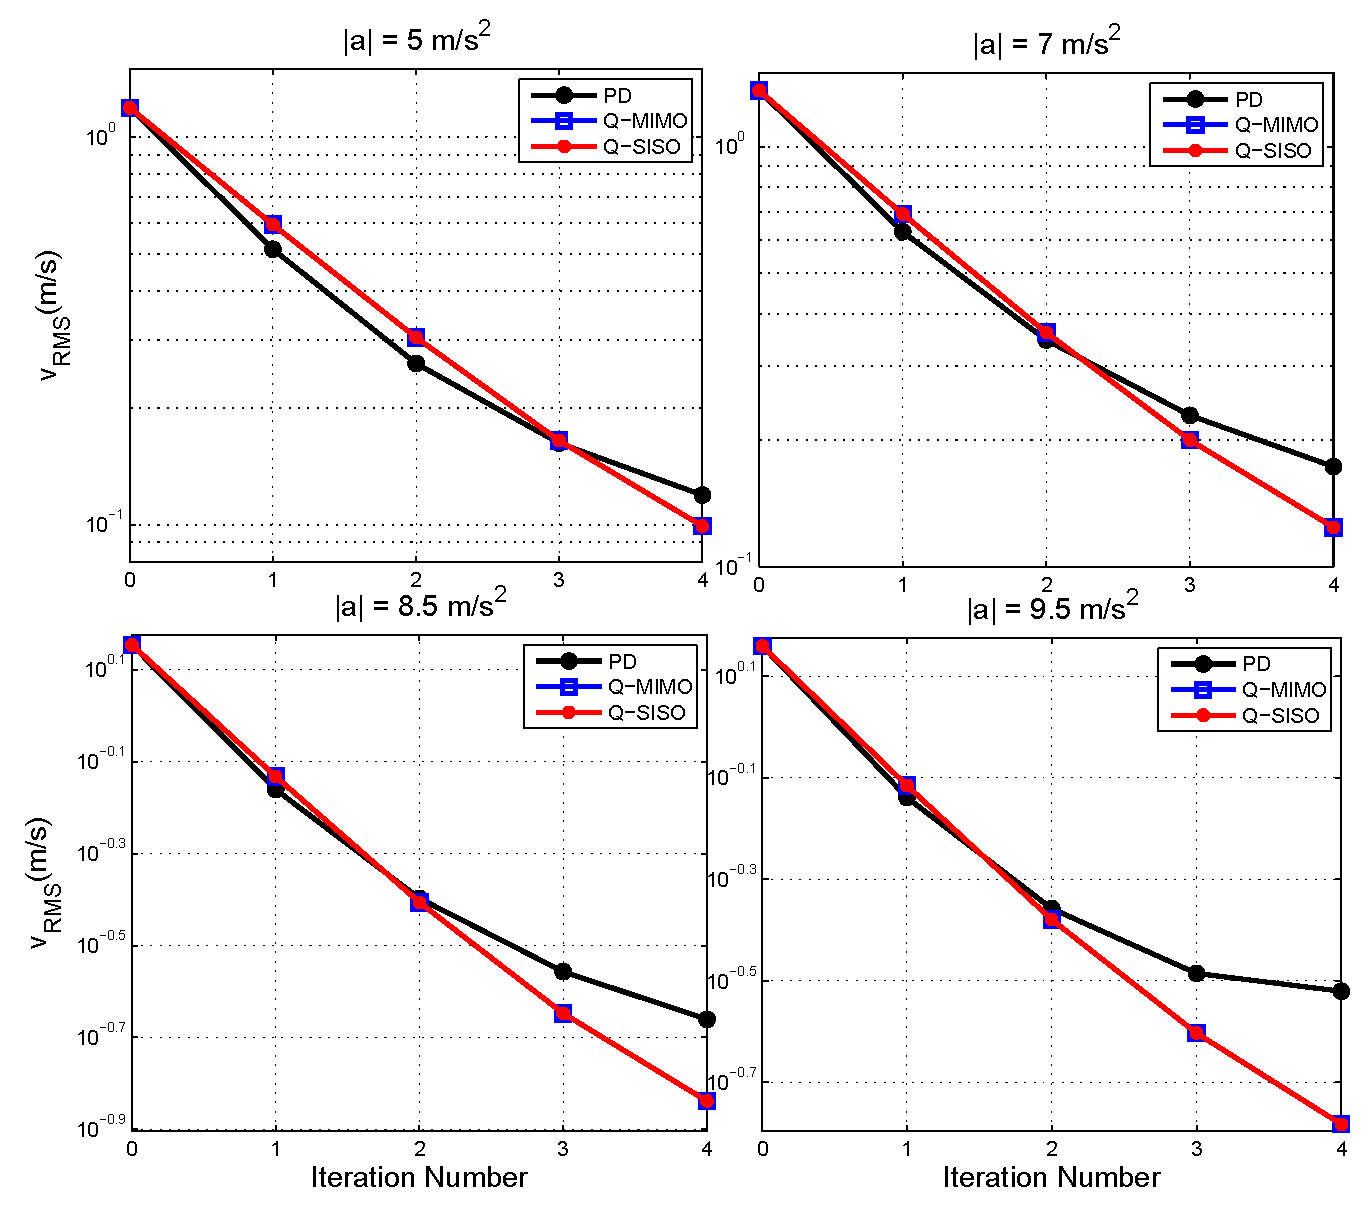
\includegraphics[width=3.5in]{figures/simRes2.eps}
\caption[Simulated results for root-mean-square speed tracking error $v$ at several values of vehicle acceleration.]{Simulated results for root-mean-square speed tracking error $v$ at several values of vehicle acceleration, with $T = I$, $R = 0$, and $S = \mathrm{1e-7} I$.
Results are plotted on a log scale.}
\label{fig:simRes2}
\end{figure}

A final comment is that the proportional-derivative ILC algorithm performs relatively poorly. At low accelerations, the
speed and path tracking performance both improve initially, but fail to improve after the second learning iteration. At high
lateral and longitudinal accelerations, the tracking performance becomes even worse for the steering ILC in Fig.~\ref{fig:simRes1}.  
This is unsurprising given that the linearized plant dynamics $P$ are not explicitly accounted for in the selection of the PD gains. 

% While the point mass model for the longitudinal dynamics is a relatively simple first order model, the lateral dynamics 
% are fourth order and highly speed dependent. A simple PD approach for learning control is likely insufficient at the limits of handling.

\subsection{Experimental Results}
\label{sec:ch4ExpRes}

Experimental data for iterative learning control was collected over four laps at Thunderhill Raceway with the autonomous Audi TTS
described in Fig.~\ref{fig:carpic}. The controller parameters are shown in Table \ref{tb:ilcprm}. 

% \begin{figure}[h]
% \centering
% 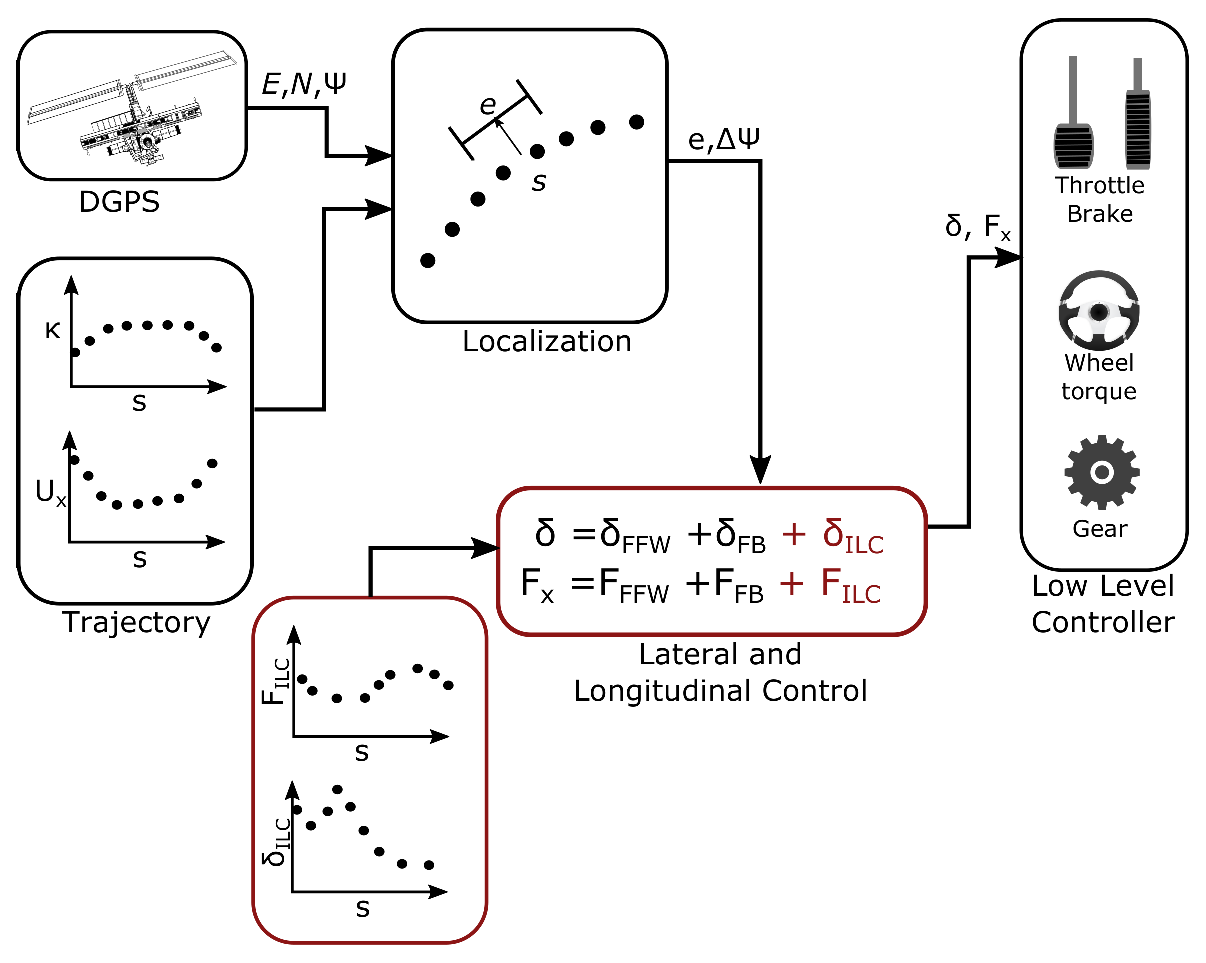
\includegraphics[width=3.5in]{figures/expSetupC4.eps}
% \caption{Controller setup for experimental testing of iterative learning control. The differential GPS (DGPS) returns global coordinates}
% \label{fig:C4setup}
% \end{figure}

\begin{table}[tb]
\begin{center}
\caption{Vehicle Parameters}\label{tb:ilcprm}
\begin{tabular}{lccc}
Parameter & Symbol & Value & Units \\\hline
Lookahead Distance       & $x_\mathrm{LA}$          &  15.2 & $\mathrm{m} $ \\
Lanekeeping Gain         & $k_{\mathrm{LK}}$         & 0.053 & $\mathrm{rad\,m^{-1}}$\\
Lanekeeping Sample Time  & $t_s$                        & 0.005 & s\\
ILC Sample Time          & $T_s$                        & 0.1   & s\\
Speed Tracking Gain                & $K_x$           & 2500 & $\mathrm{Nsm^{-1}}$\\
Q-ILC Matrix (Path)            & $T$ and $R$              &  $I$      & - \\
Q-ILC Matrix  (Path)           & $S$                       & 100\,$I$  & - \\
Q-ILC Matrix (Speed)            & $T$              &  $I$      & - \\
Q-ILC Matrix (Speed)            & $R$              &  $0$      & - \\
Q-ILC Matrix  (Speed)           & $S$                       & 1e-7\,$I$  & - \\\hline
\end{tabular}
\end{center}
\end{table}


Fig.~\ref{fig:expRes1} shows the applied iterative learning signals and resulting path tracking error over four laps using the SISO
quadratically optimal learning algorithm. The car is driven
aggressively at peak lateral/longitudinal accelerations of 8 $\mathrm{m/s^2}$. On the first lap, despite the 
incorporation of a feedforward-feedback controller operating at a high sampling rate, several spikes in tracking error are visible due to transient vehicle dynamics.

However, the iterative learning algorithm is able to significantly attenuate these transient spikes after just two or three laps. One of the most important features of the time series plot is that the learned steering corrections are applied slightly before a lateral path deviation was observed the prior lap (i.e. the steering corrections \textit{lead} the observed error). This is because the ILC learns to anticipate repetitive disturbances and acts proactively.

\begin{figure}[h!]
\centering
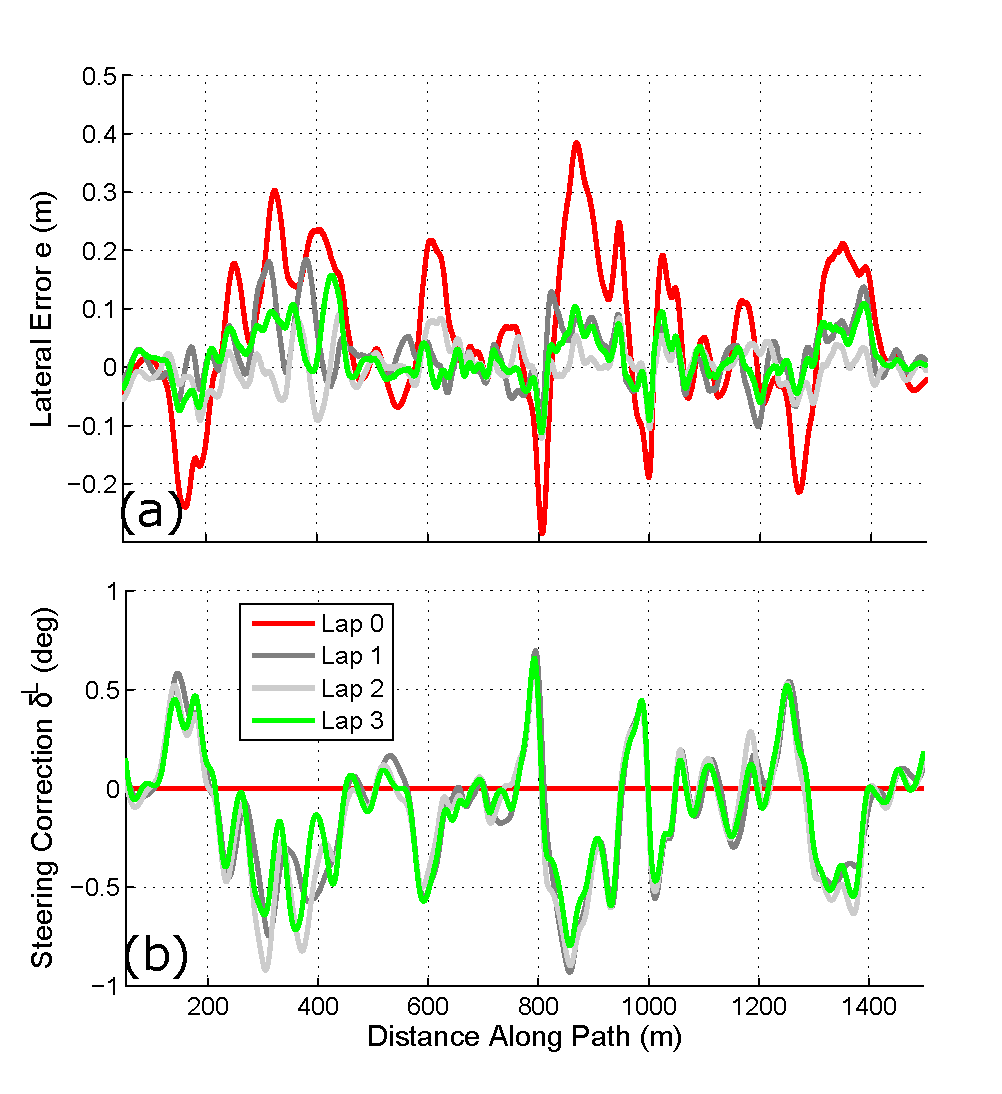
\includegraphics[width=3.5in]{figures/expRes1.eps}
\caption{Experimental results for path tracking error with Q-SISO learning controller, at peak lateral accelerations of 8 $\mathrm{m/s^2}$.}
\label{fig:expRes1}
\end{figure}

\begin{figure}
\centering
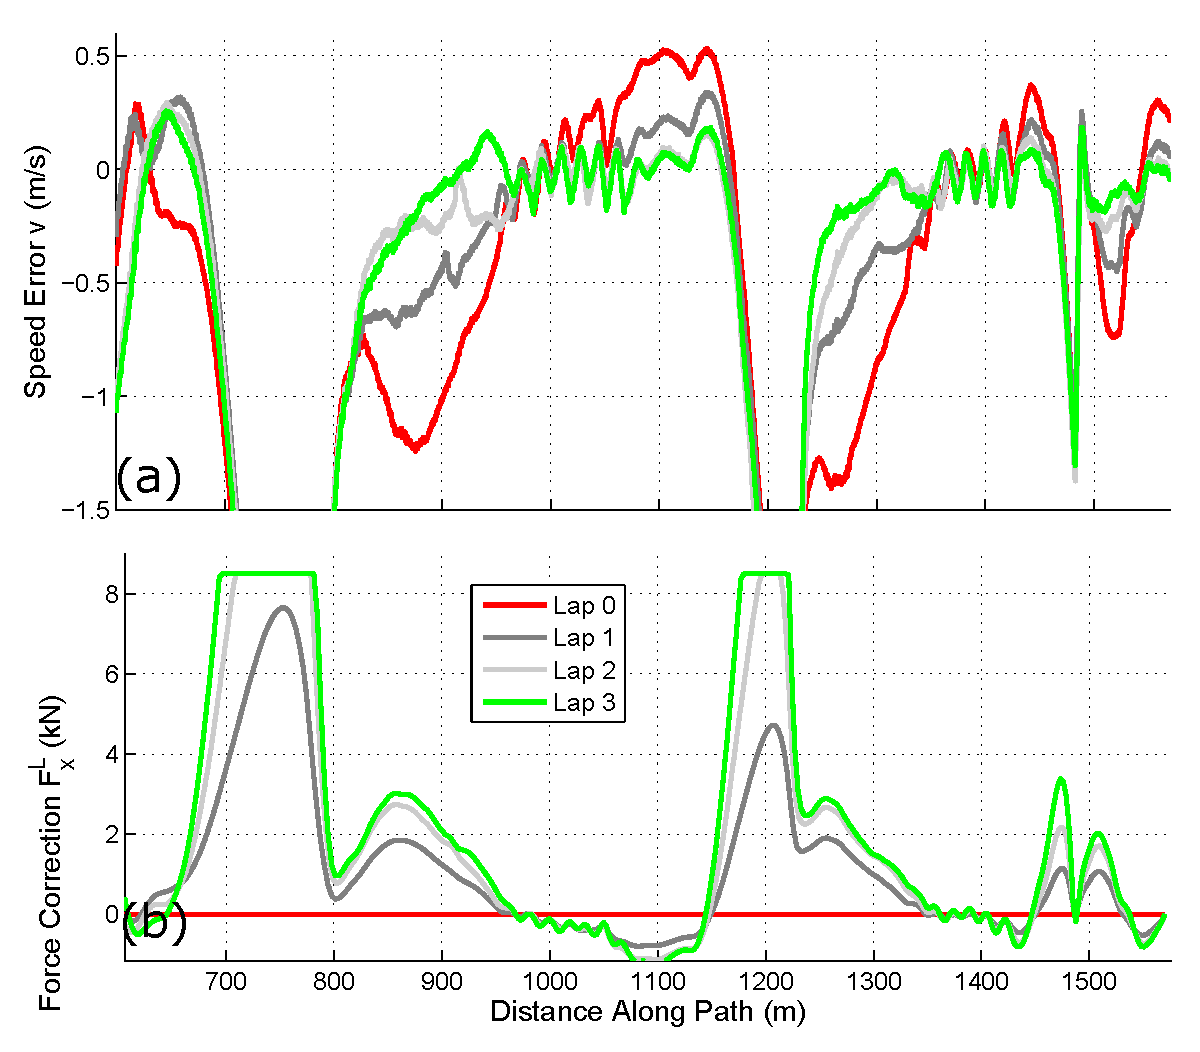
\includegraphics[width=3.4in]{figures/expRes2.eps}
\caption{Experimental results for speed tracking error with Q-SISO learning controller, at peak lateral accelerations of 8.5 $\mathrm{m/s^2}$.}
\label{fig:expRes2}
\end{figure}

Fig.~\ref{fig:expRes2} shows the iterative learning signals for the longitudinal speed control at a slightly
higher acceleration of 8.5 $\mathrm{m/s^2}$. Again, in just
two to three iterations, significant lags in the speed tracking are attenuated from $s = 800-900$ meters and $s = 1200-1300$ meters. 

% Additionally, the controller also acts to slow the car down when $v > 0$ and the vehicle exceeds the speed profile. This is also desirable
% from a racing perspective as it it prevents the vehicle from exceeding the friction limit. Oscillations in speed tracking
% performance are visible in Fig.~\ref{fig:expRes1}(a) from 900 - 1100 meters and 1300 - 1400 meters. These are generally undesirable, and further tuning of the filter matrix $Q$ is possible
% to remove rapid changes in the learned force input. 
 
 Notice that Fig.~\ref{fig:expRes2} has
several regions where the speed error $v << 0$. These are straight regions of the track where is no true planned speed
because the desired longitudinal action is to fully apply the throttle and go as fast as physically possible. For convenience, the ILC is programmed to saturate the longitudinal
learning signal to 8000 Newtons. This is unlikely to affect convergence as the throttle is likely to already be fully applied. 

% , although a more elegant solution is to switch the ILC controller off on straight portions of the track. 

In Fig.~\ref{fig:expRes3}, root-mean-square tracking results are shown for a range of peak vehicle accelerations. 
The results show that at lower vehicle accelerations,
the initial speed and lateral tracking errors (Iteration 0) are smaller, as the built-in feedback-feedforward controller 
performs better. However, as the speed profile becomes more aggressive, the path and speed tracking degrades in the presence
of highly transient tire dynamics. Regardless of the initial error, application of iterative learning control 
reduces the trajectory tracking errors significantly over just 2 or 3 laps. At an acceleration of 8.5 $\mathrm{m/s^2}$, for example, the RMS
lateral tracking error is around 3 cm, on the order of the expected RMS error from the GPS position sensor. 

On some tests, the RMS tracking error 
increases slightly from
Lap 2 to Lap 3, and for the case where vehicle acceleration is 9 $\mathrm{m/s^2}$, the lateral tracking error is constant from Lap 1 to Lap 2
before decreasing further in Lap 3. While not predicted in simulation, this behavior likely occurs because the repeating disturbance
from lap-to-lap is not exactly constant, especially as the vehicle approaches the handling limits. 

% More refined tuning of the gain matrices may be able to prevent 
% this RMS error increase, or the ILC algorithm can be stopped after several iterations once the tracking performance is acceptable.

% Experimental results in this section were only given for the quadratically optimal controller with decoupled (SISO) dynamics. 
% The PD iterative learning controller was not tested due to the relatively worse simulation performance, and the quadratically optimal controller with coupled dynamics provided no clear benefit in simulation but a much longer computation time. 



\begin{figure}
\centering
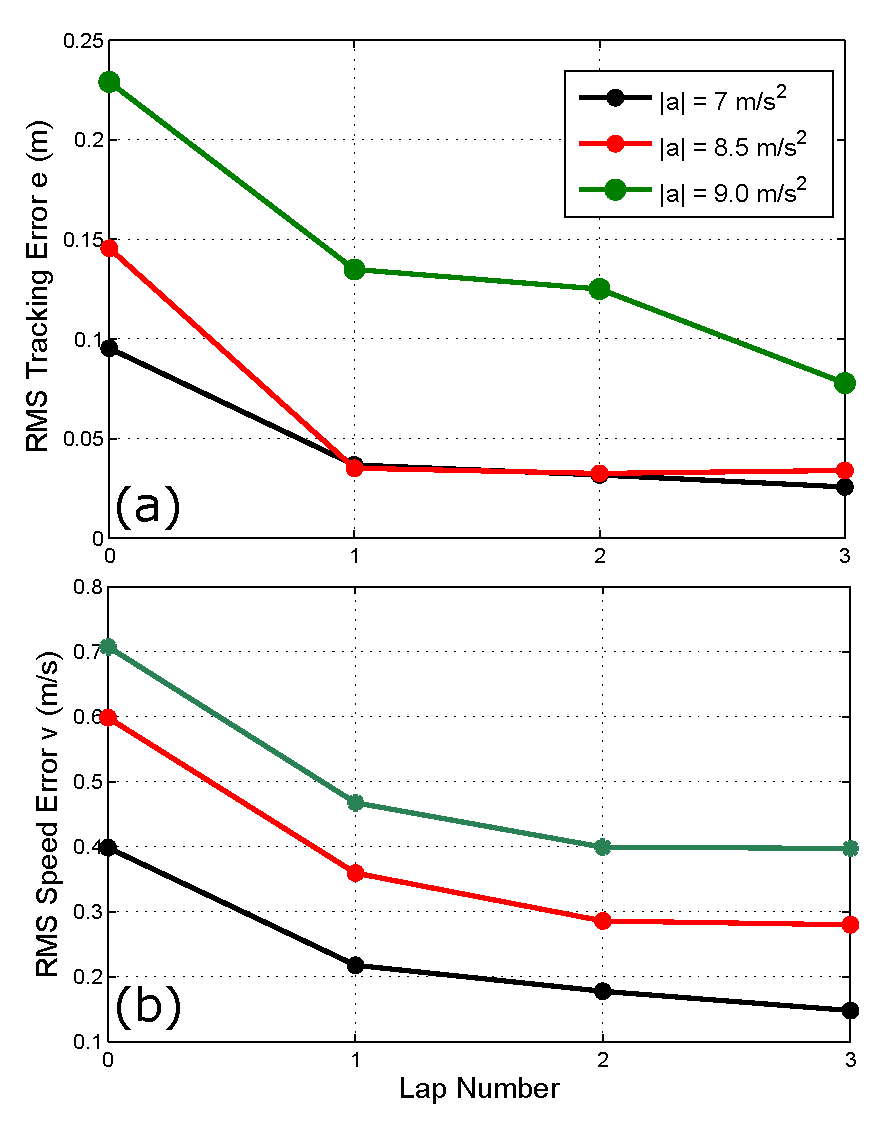
\includegraphics[width=2.8in]{figures/expRes3.eps}
\caption[Experimental RMS tracking error for the Q-SISO learning controller at several levels of lateral acceleration. ]{Experimental RMS tracking error for the Q-SISO learning controller at several levels of lateral acceleration. (a) RMS lateral tracking
error as a function of lap number/iteration number. (b) RMS speed tracking error as a function of lap/iteration number. Note that lap 0 corresponds
to the baseline case where iterative learning control is not applied.}
\label{fig:expRes3}
\end{figure}

\section{Iterative Trajectory Modification}
\subsection{Effect of Tire Slip Norm on Lap Time}
\label{sec:etu}

Fig.~\ref{fig:t2} shows the complicated effect of driving at different levels of lateral and longitudinal acceleration for region \circled{2} in Fig.~\ref{fig:expErrors}. Recall that the
speed profile is generated by assuming a global value of tire friction $\mu$, which is directly related to the acceleration norm of
the desired speed profile $\left(\sqrt{a_x^2 + a_y^2}\right)$ by a factor of \mbox{$g =$ 9.81 $\mathrm{m/s^2}$}. 

% Fig.~\ref{fig:t2}(a) confirms that higher levels
% of $\mu$ result in strictly faster speed profiles for the same turn. 

\begin{figure}
\centering
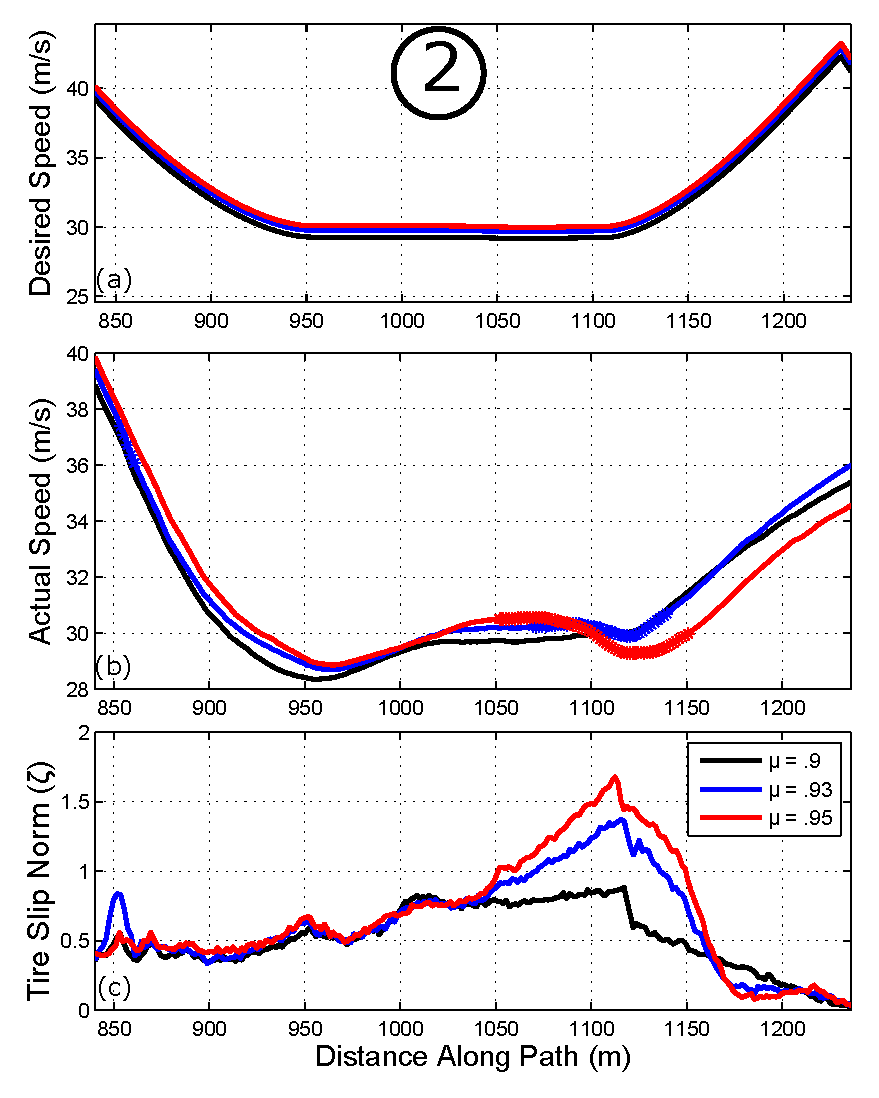
\includegraphics[width=2.3in]{figures/t2res.eps}
\caption[Desired speed for varying levels of $\mu$ - region 2]{(a) Desired speed for varying levels of $\mu$ (b) Actual speed for varying levels of $\mu$. Asterisks correspond to 
regions where $\zeta > 1$. (c) Tire slip norm for varying levels of $\mu$. }
\label{fig:t2}
\end{figure}

However, selecting a more aggressive value of $\mu$ does not necessarily entail a faster experimental lap time. Consider the actual speeds of the vehicle in
Fig.~\ref{fig:t2}(b) when trying to experimentally follow three different speed profiles. For the case where $\mu = 0.9$, the vehicle completes
the turn without fully utilizing the tire's capability and achieves relatively low velocities. For the extreme case where $\mu = 0.95$, the
vehicle enters the turn at a high speed but then begins to slide as $\zeta = 1.6$. While not shown in the plot, the saturation
is occurring primarily at the front tires, causing an understeer that can cause the car to skid off the track. Completing the lap therefore requires a stabilizing
action from the stability controller to slow the car down and regain control of the vehicle. 

As a result,
when the vehicle accelerates at the end of the turn, the actual vehicle speed at $\mu = 0.95$ is significantly slower than the case where $\mu = 0.9$.
A final ``just right" value of $\mu = 0.93$ was also tested experimentally for this turn, and while the car does slide a bit at this level of driving (peak $\zeta = 1.3$),
the needed stabilizing action is significantly smaller and the vehicle exits the turn with the highest speed. 

%  \begin{figure}[tb]
% \centering
% 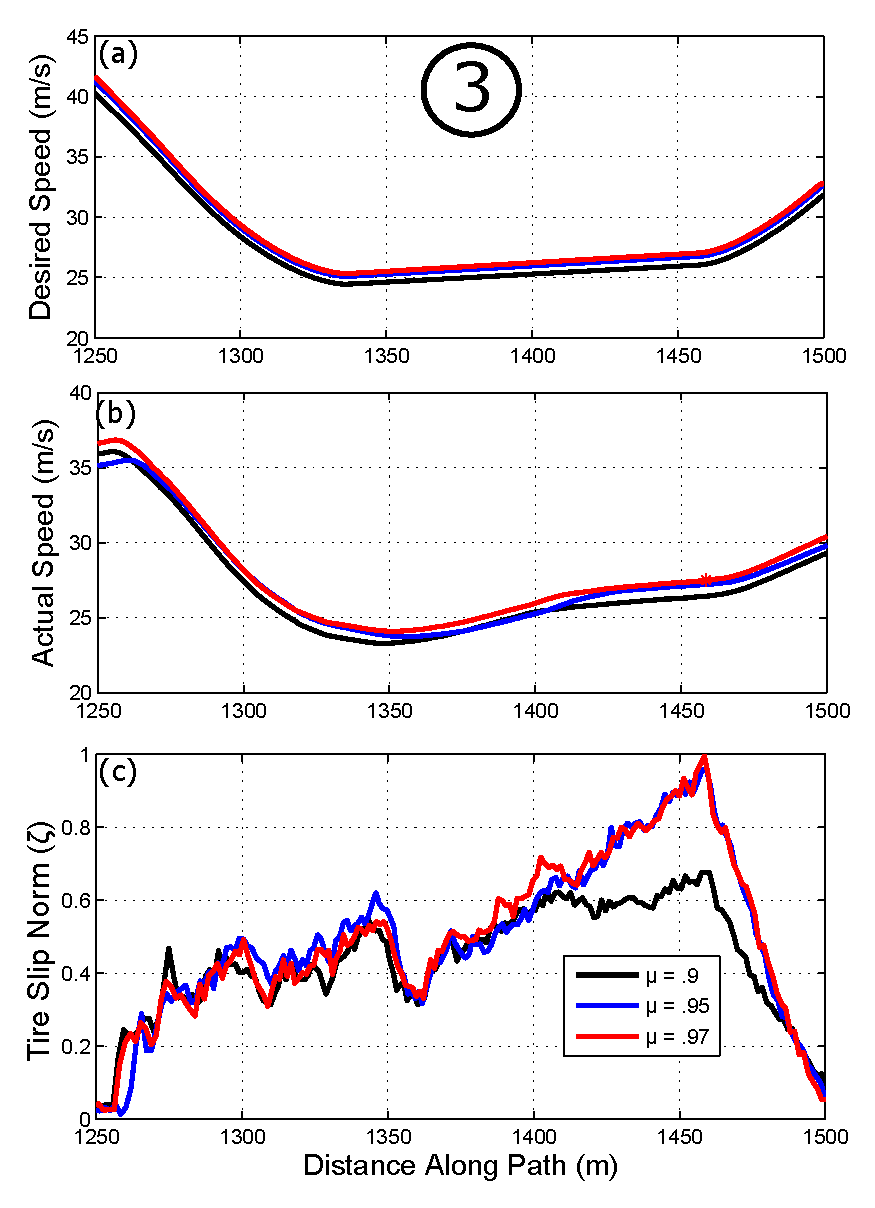
\includegraphics[width=2.3in]{figures/t3res.eps}
% \caption[Desired speed for varying levels of $\mu$ - region 3]{(a) Desired speed for varying levels of $\mu$. (b) Actual speed for varying levels of $\mu$. Asterisks correspond to 
% regions where $\zeta > 1$. (c) Tire slip norm for varying levels of $\mu$. }
% \label{fig:t3}
% \end{figure}

% Unfortunately, the best value of $\mu$ is not constant throughout the track. Fig.~\ref{fig:t3} 
% shows the same data plotted for region \circled{3} of the 
% Thunderhill Raceway. In this case, even with an atypically high value of 
% $\mu = 0.97$, the slip norm of the vehicle tires is relatively low, and the value of $\mu$ that optimizes the completion time for this turn could 
% be even larger. 


\subsection{Naive Method: Greedy Algorithm}
\label{sec:greedy}

Section \ref{sec:etu} shows that to  minimize the overall lap time, there is a need to generalize the speed profile such that different portions of the track can be driven with different
values of $\mu$. In other words, \textbf{the problem is to learn the ``friction profile" $\mu^\star(s)$ along the path that minimizes the experimental vehicle lap time.} 

The simplest approach to finding $\mu(s)$ is a greedy algorithm where a set of experimental data is collected for a variety of different speed profiles, each corresponding to a different value of $\mu$ and therefore a different acceleration level. The greedy approach is then to discretize the track into a number of small sections and pick the value of $\mu$ for each section that corresponds to the highest observed experimental velocity.
The final desired velocity profile is then generated using the numerical integration approach presented in \cite{subosits2015autonomous}. This method does not require a single 
value of friction across the whole track, and generates a smooth velocity profile even when the peak acceleration limits vary from point to point. 

 \begin{figure}[tb]
\centering
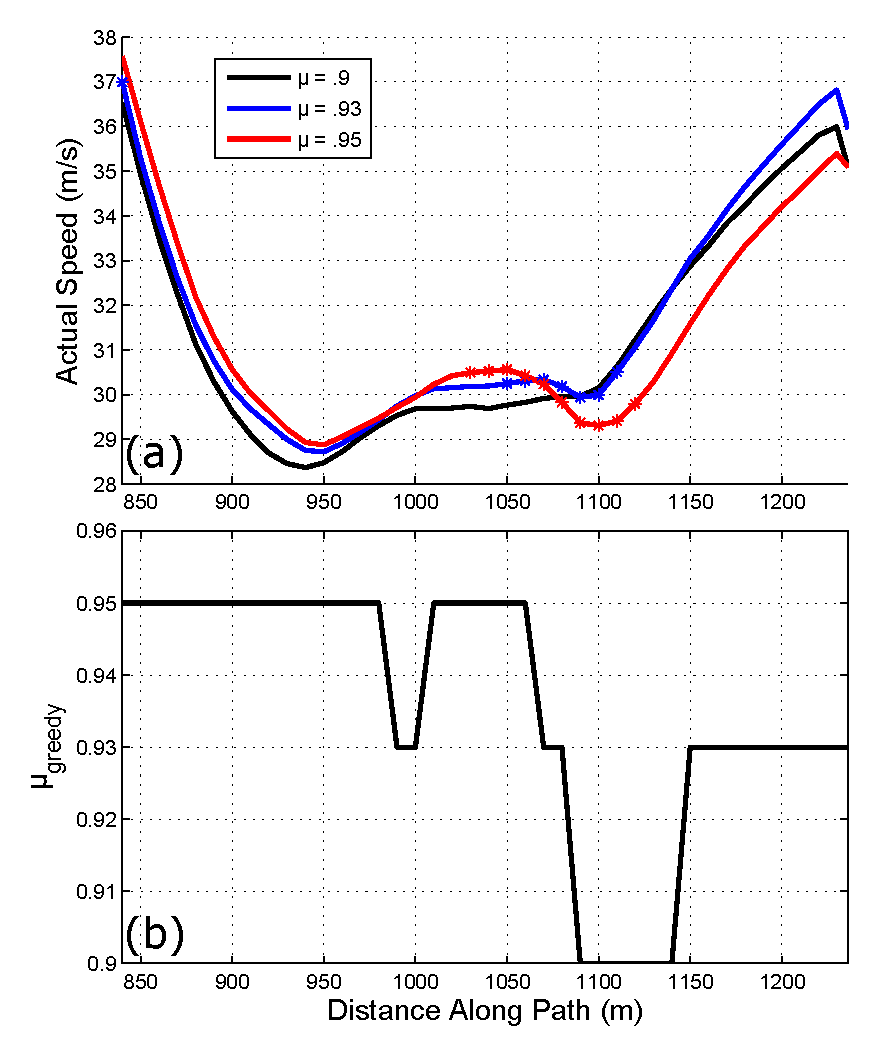
\includegraphics[width=2.8in]{figures/turn2greedy.eps}
\caption[Greedy algorithm results for region 2.]{(a) Desired speed for varying levels of $\mu$ (b)``Greedy" value of $\mu$ as a function of distance along track. Asterisks denote
region of track where vehicle is understeering.}
\label{fig:t2g}
\end{figure}

A plot showing the results of applying the greedy algorithm for section \circled{2} is shown in Fig.~\ref{fig:t2g}. The flaw in simply selecting $\mu$ based on the highest speeds is apparent at $s = 1050 \mathrm{m}$. The greedy algorithm suggests the vehicle mostly drive at $\mu$ = 0.95,
but then switch to driving at $\mu = 0.93$ as soon as the vehicle begins to slide. Switching to a less aggressive velocity profile at this point is impossible to achieve in practice, because the vehicle is already fully sliding and has no control until the vehicle slows down.

 % As a result, the greedy algorithm fails to capture the hidden cost of a large understeer, which results in a period of time where the speed must inevitably drop. 

\subsection{Framing Trajectory Learning as Search Problem}
\label{sec:framingTL}

Given the inadequacy of the greedy algorithm, a more sophisticated approach is necessary to learn $\mu^\star(s)$ from
experimentally observed data. This section frames the desire to find the minimum time $\mu^\star(s)$ as a tree search problem.
Consider discretizing the racing path into $N$ evenly spaced segments. For example, on the Thunderhill Raceway with
$\Delta s = 5 \mathrm{m}$, $\textbf{s} = [0 \hspace{2mm} 5 \hdots s_k \hdots 4495 \hspace{2mm} 4500]$ for $k = 0 \hdots N$, with $N = 901$. For each
path distance $s_k$, there are $M_k$ velocity and $M_k$ tire slip observations from experimental data, each corresponding to a different $\mu$. 
For example, looking at Fig.~\ref{fig:t2}, if $k = 191$, $s_k =  950 \mathrm{m}$, $M_k = 3$, the velocity and slip norm $\zeta$ observations $U_k(\mu)$ and $Z_k(\mu)$ are shown in Table \ref{tb:Uk}:

\begin{table}[h]
\begin{center}
\caption{$U_k(\mu)$ and $Z_k(\mu)$ for $k =$ 191}\label{tb:laptimes}
\begin{tabular}{ccc}
\label{tb:Uk}
$\mu $&$ U_x(m/s) $& $\zeta $\\\hline
0.9 & 28.42 & 0.55\\
0.93& 28.91 & 0.63\\
0.95& 29.14 & 0.66\\\hline
\end{tabular}
\end{center}
\end{table} 
 $M_k$ is not necessarily the same for all $k$ to account for experimental trials that do not cover the full lap. For safety and time
 reasons, some parts of the track will only have experimental data collected at two different friction values, while others may have five or six.

 Nodes of the search tree are then defined as a two-element state tuple, with the first state element being $s_k$ and the second element being the current
 friction coefficient $\mu_k$. Since the car must start from the beginning of the path, the first state has $s_0 = 0$.
 The $M_k$ edges from a given node correspond to actions that the car can take at $s = s_k$. In this case, the ``action" is the next value of $\mu$,
 and the successor states are $(s_{k+1}, \mu_1) ... (s_{k+1}, \mu_{M_k})$. A diagram of the search tree is shown in Fig.~\ref{fig:stree}.

\begin{figure}
\centering
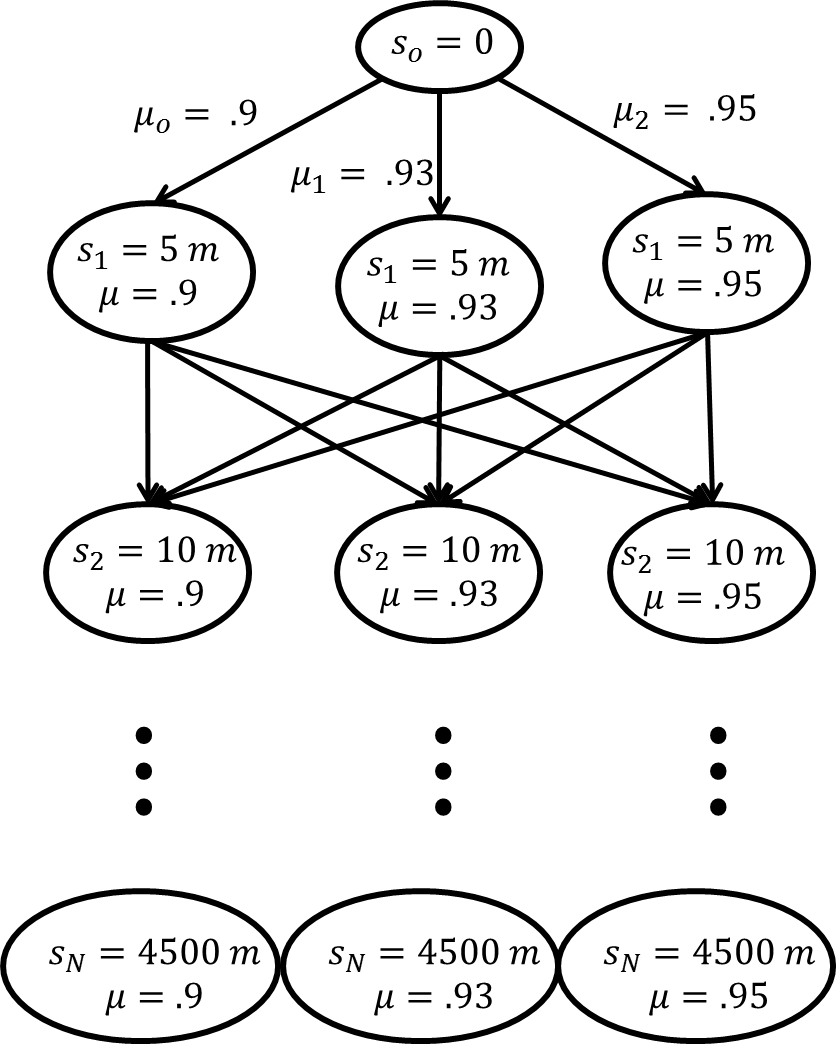
\includegraphics[width=2.2in]{figures/searchTree.png}
\caption{Sample search tree for Thunderhill race track where there are only 3 experimentally observed full laps at $\mu =$ 0.9, 0.93, 0.95.}
\label{fig:stree}
\end{figure} 

 
Each edge is associated with a travel cost $c_t$. The travel cost for a given edge is the amount of time it takes to go from
$s = s_k$ to $s = s_{k+1}$ driving at the friction coefficient $\mu$ associated with that edge. As illustrated in Fig.~\ref{fig:costDiag}, the cost is estimated from the experimentally
observed data assuming linear acceleration between points. The travel cost from node $(s_k, \mu_k)$ to $(s_{k+1}, \mu_{k+1})$ can therefore be expressed mathematically with trapezoidal integration of the straight-line velocity profile:
\begin{align}
c_t(s_k, s_{k+1},\mu_k, \mu_{k+1}) &= \ln \frac{a_x(\Delta s) + U_k(\mu_k)}{a_x} - \ln \frac{U_k(\mu_k)}{a_x} \\
a_x &= \frac{U_{k+1}(\mu_{k+1}) - U_k(\mu_k)}{\Delta s}
\end{align}

 \begin{figure}[tb]
\centering
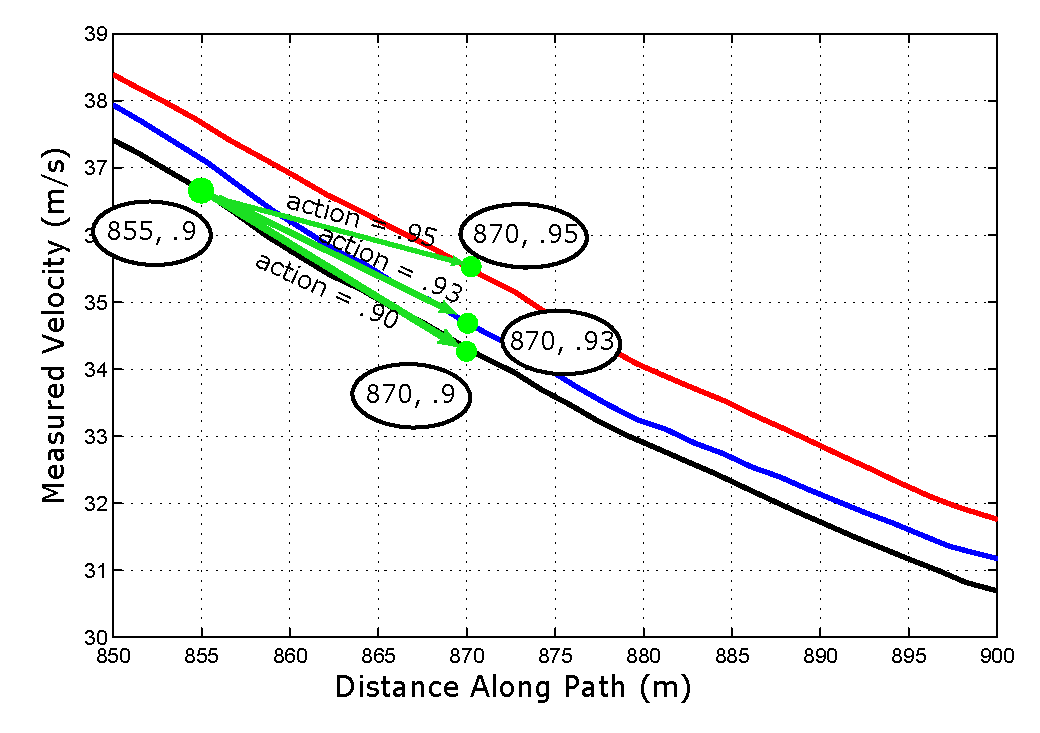
\includegraphics[width=3in]{figures/costStructure.eps}
\caption[Illustration of travel cost.]{Illustration of travel cost. Current state is (855, 0.9). Assuming $\Delta s$ is 15 meters, cost is time to travel from this node
to one of the three possible successor nodes, depending on the action taken.}
\label{fig:costDiag}
\end{figure} 

In addition to the travel cost, there is also a \textit{switching} cost $c_s$ associated with switching to a different value of $\mu$. These
are determined by the observed tire slip norm measurements $Z_k(\mu)$. The switching cost is expressed mathematically as:

\begin{align}
\label{eq:swCost}
c_s(s_k, s_{k+1},\mu_k, \mu_{k+1}) &= \\
&\mathds{1}\left(\mu_{k+1} \neq \mu_{k}\right)\left(\lambda  + \infty \times\mathds{1}\left(Z_k(\mu_k) > 1\right) \nonumber \right)
\end{align}

Where $\mathds{1}$ is the indicator function. The switching cost function (\ref{eq:swCost}) implies that an action will never
incur a switching cost if the selected value of $\mu$ is unchanged from the previous selection. If the value of $\mu$ does change, there
is a small switching penalty $\lambda$, chosen by trial and error to discourage the search algorithm from changing the friction profile to gain a
trivial decrease in lap time. Additionally, there is a very large (infinite) switching penalty if the search algorithm attempts to change the
friction profile while the vehicle's tires are saturated ($\zeta > 1$). This reflects the physical inability of the car to control its
trajectory while sliding and is what separates the search algorithm from the greedy algorithm. A diagram demonstrating (\ref{eq:swCost})
is shown in Fig.~\ref{fig:swCost}. 

 \begin{figure}[tb]
\centering
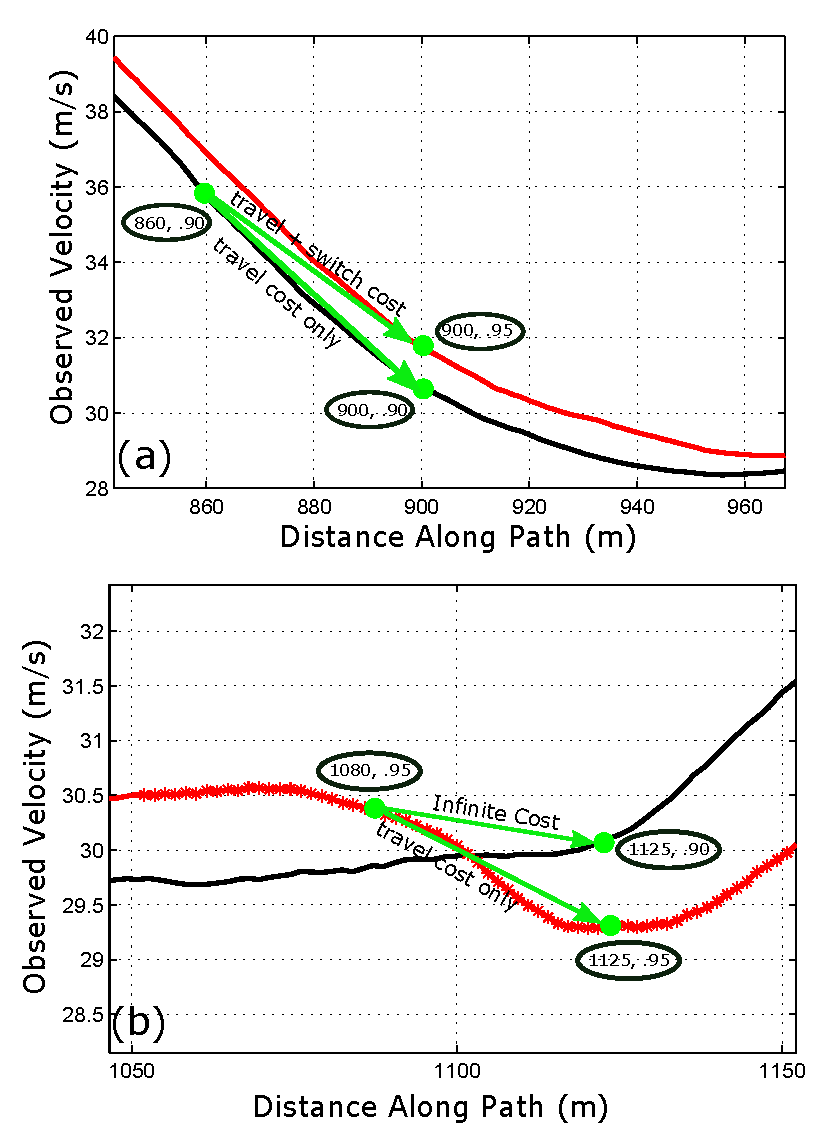
\includegraphics[width=2.5in]{figures/switchCost.eps}
\caption[Costs when vehicle is and is not sliding.]{(a) Costs when vehicle currently is not sliding. The vehicle can switch to a more aggressive velocity profile, paying a small
switching penalty, or can continue on the current profile. (b) Costs when vehicle is currently sliding. Vehicle has no choice but to continue on current
trajectory. Asterisks denote regions where $\zeta > 1$ and the vehicle is sliding.}
\label{fig:swCost}
\end{figure} 

\subsection{A* Search Algorithm and Heuristic}
\label{sec:ch5astarheuristic}

Once the tree is mathematically defined in terms of the start state, nodes, edges, and costs, the search problem is to find the sequence
of actions from the start node to any terminal node that minimizes the total cost. In our case, the start state, nodes, edges
and costs were defined in the previous section, and a terminal node is any node at the end of the path (i.e. $k = N$). The sequence
of actions in our case is the friction profile $\mathbf{\mu} = [\mu_1 \hdots \mu_k \hdots \mu_N]$, which determines how
aggressively the vehicle will drive on every part of the track. The total cost is the sum of all individual travel costs $c_t$ and switching costs
$c_s$, and has intuitive units of time. 

% Minimum-cost tree spanning algorithms (e.g. breadth-first search, Dijkstra's algorithm, etc.) are a well known subject and a thorough description
% can be found in \cite{aibook}.

 For the purpose of solving this search problem, the A* search algorithm is used. 
Like breadth-first search, the A* algorithm is guaranteed to find the lowest cost path from a start node to a goal node, 
but uses a priority queue data structure to more efficiently explore the search tree. Frontier leaf nodes $n$ being
considered for exploration are ranked according to the following modified cost:

\begin{equation}
f(n) = g(n) + h(n)
\end{equation}
where $g(n)$ is the true cost to go from the start node to node $n$. The function $h(n)$ is a heuristic estimate of the cost to get from node $n$ to any goal state (i.e. to the end of the
path). For A* to be guaranteed to find the shortest path, $h(n)$ must be \textit{admissible}, meaning that $h(n)$ must underestimate the
true cost of getting to the end of the path. 

In our case, we have a very intuitive heuristic function $h(n)$ for the A* implementation. In Sec. \ref{sec:greedy}, the greedy approach
was discussed. Define $\mathbf{U_\mathrm{g}} = [U_\mathrm{g}(1) \hdots U_\mathrm{g}(k) \hdots U_\mathrm{g}(N)]$ to be the highest observed
experimental speed for each index $s_k$. Because we know tracking this greedy profile is physically impossible due to vehicle sliding, time estimates
from this profile will always underestimate the true cost. We therefore define $h(n)$ as follows:

\begin{equation}
\label{eq:heuristic}
h(n) = \int^{s_N}_{s_n} \frac{1}{U_g(s)} ds
\end{equation}
where $s_n$ is the value of $s$ corresponding to node $n$ and $s_N$ is the total length of the track. While (\ref{eq:heuristic}) is an integral equation, it can be solved for the discrete
array $\mathbf{U}_\mathrm{g}$ via trapezoidal numerical integration.

\subsection{A* Implementation and Results}

Because the A* algorithm relies on experimental observations to learn $\mu^\star(s)$, experimental data was collected over several trials, with
each trial consisting of a speed profile generated with a constant $\mu$ value over the track. The $\mu$ values chosen for
experimental data collection were 0.85, 0.9, 0.92, 0.93, 0.94, 0.95, and 0.97. 

Due to safety and time constraints associated with collecting high speed race data, only the speed profiles corresponding to $\mu = 0.92$ and $\mu = 0.94$ were observed
over the whole track. The other speed profiles were only tested on critical sections of the track. 

% Fig.~\ref{fig:muCoverage} shows the experimental data coverage. 

\begin{table}[h]
\begin{center}
\caption{Search Algorithm Information}\label{tb:astarparams}
\begin{tabular}{lccc}
Parameter & Symbol & Value & Units \\\hline
Track Length       & $L$           &  4500 & $\mathrm{m} $ \\
Discretization Length               & $\Delta s$  & 5 & $\mathrm{m}$\\
Number of Points  & $N$                        & 901 & -\\
Switching Cost          & $\lambda$                        & 0.05   & s\\\hline
CPU Solution Time           &                                  &  70    & s \\
Nodes Explored              &                                  &  6887  & - \\\hline
\end{tabular}
\end{center}
\end{table}

%  \begin{figure}[tb]
% \centering
% 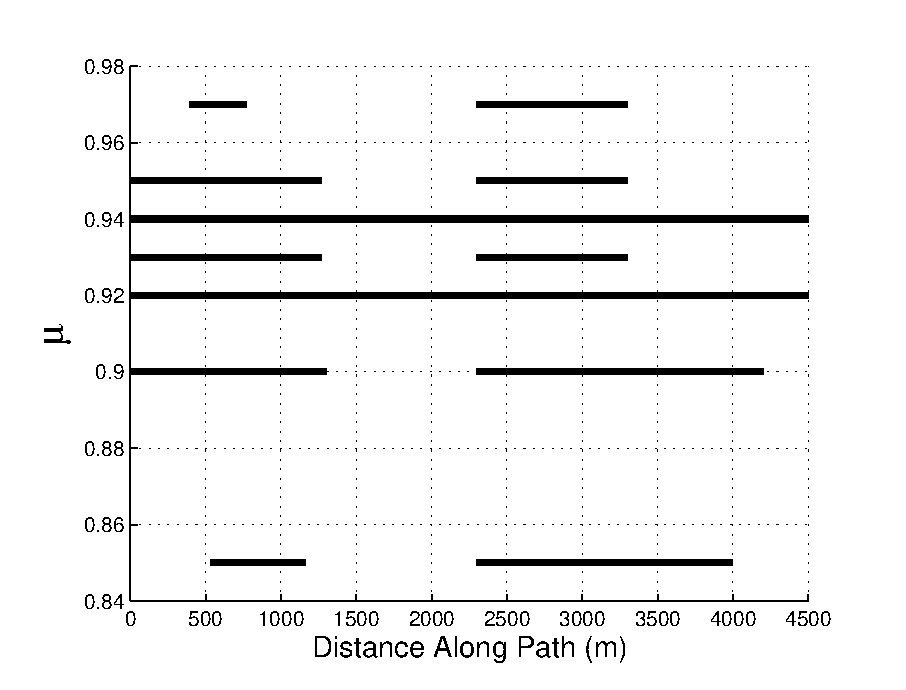
\includegraphics[width=2.45in]{figures/muCoverage.eps}
% \caption[Coverage of experimental data]{Coverage of experimental data. For speed profiles corresponding to $\mu = 0.92$ and $\mu = 0.94$, experimental data of the autonomous race vehicle was observed
% over the whole track. For safety and time constraints, the other speed profiles were only tested on sections of the track.}
% \label{fig:muCoverage}
% \end{figure} 

% After collecting the experimental data, the A* algorithm was applied to learn the optimal friction profile $\mu^\star(s)$. Parameters for the algorithm are shown in Table~\ref{tb:astarparams}. To interface more efficiently with experimental data files, the search algorithm was implemented in MATLAB using custom code instead of a standard search algorithm library. The entire search process took approximately 70 seconds on a core i7 laptop machine, exploring 6887 nodes in the process. However, since MATLAB is not designed for computational efficiency in tree-based search algorithms, a C++ implementation would likely
% be several orders of magnitude faster. 

 The resulting $\mu^\star(s)$ profile associated with the minimum lap time on Thunderhill Raceway is shown in Fig.~\ref{fig:muprof}. For  comparison, the A* solution is plotted against the greedy algorithm solution. Because of the incorporation of switching costs,  the A* algorithm switches $\mu$ values only when necessary to achieve a nontrivial increase in lap time, and only switches $\mu$ when  the vehicle is not sliding. The same results are plotted on a map of the track in Fig.~\ref{fig:mumap}. A satisfying observation is that the optimal profile reduces $\mu$ to 0.93 in section \circled{2} to be more conservative. This matches our observations about tire slip norm $\zeta$ in Sec.~\ref{sec:etu}. 
 
 Predicted lap time results are shown in Table~\ref{tb:predresults}. Notice that the A* predicted lap time is slightly
 slower than the greedy algorithm prediction, which is expected given the physical infeasability of the greedy algorithm assumptions. The  results also indicate that a significant lap time improvement can be expected over a velocity profile generated with a constant $\mu$.
 
 \begin{figure}[tb]
\centering
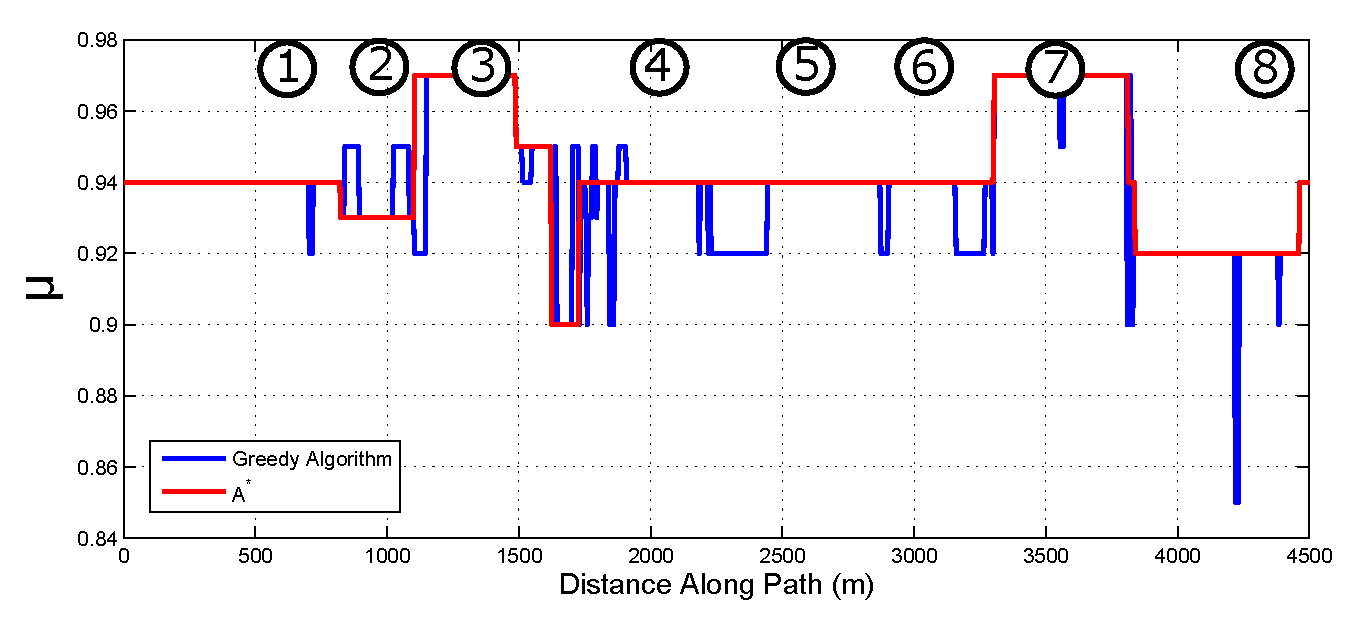
\includegraphics[width=2.8in]{figures/muprofile.eps}
\caption{Minimum time $\mu(s)$ profile for Thunderhill, for both the A* solution and greedy algorithm solution.}
\label{fig:muprof}
\end{figure}  

 \begin{table}[h]
\begin{center}
\caption{Lap Times}\label{tb:predresults}
\begin{tabular}{l|c}
Driver          & Lap Time \\\hline
Constant $\mu(s)$ = 0.94 & 139.2 \\
Constant $\mu(s)$ = 0.92 & 139.4 \\\hline
Greedy $\mu_g(s)$ (Prediction) & 136.4 \\
A*     $\mu^*(s)$ (Prediction) & 136.8 \\\hline
\end{tabular}
\end{center}
\end{table}
 
\begin{figure}[tb]
\centering
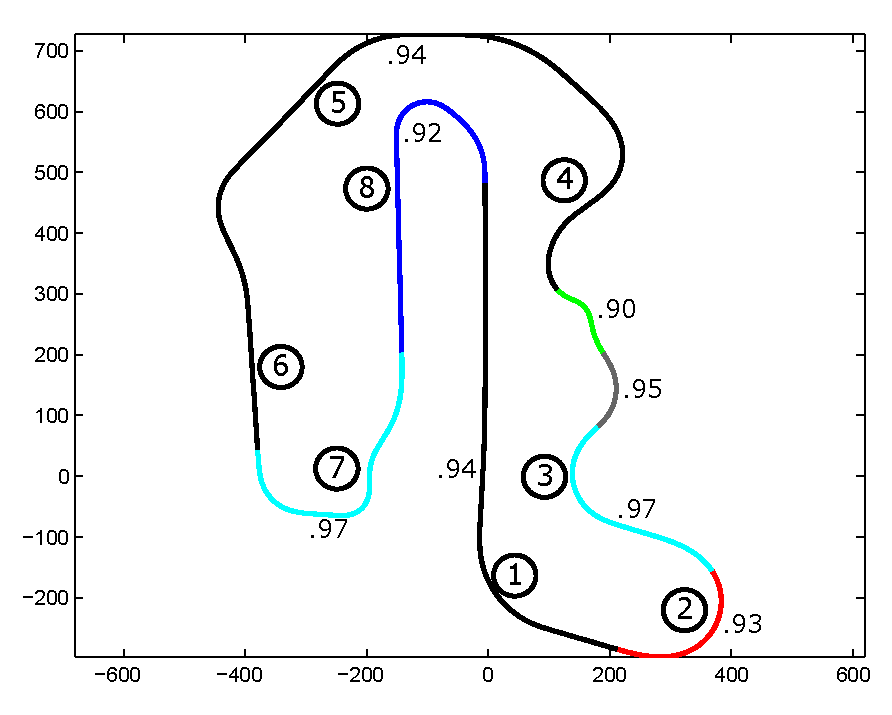
\includegraphics[width=3.5in]{figures/mumap.eps}
\caption{Minimum time $\mu^\star(s)$ profile from A* algorithm plotted on map of Thunderhill.}
\label{fig:mumap}
\end{figure}  

Fig.~\ref{fig:mumap} provides interesting insights about what the A* algorithm is learning. Section \circled{2} is a 
long, sweeping turn with mostly steady-state cornering dynamics, so the optimal friction value of .93 is in the middle
of the range of possible values and representative of the average friction between the tires and the track. Sections \circled{3}
and \circled{7} represent short turns followed by a turn in the opposite direction. For these turns, the algorithm has learned it is better to drive a little
 faster than the true friction limit would dictate, because by the time the vehicle begins to understeer, the turn is already complete and
 the vehicle can reverse the steering quickly while following the desired path. Section \circled{8} occurs before a long straight section of the track where recovering
from an understeer would result in a significantly lower speed on the fastest part of the track. As a result, the algorithm's planned acceleration is more conservative. 

% Finally, 
% the section with the lowest $\mu(s)$ occurs on a part of the track with significant lateral weight transfer. In general, lateral weight transfer reduces the cornering forces available
% to the vehicle, but this effect was not captured in the trajectory planning phase, which assumed a planar model with coupled left and right tires. In summary, the A*
% algorithm allows the car to learn subtle but important driving behaviors that are not easily captured through simulation. 

\subsection{Experimental Validation}
The best validation of the A* algorithm is to experimentally drive the optimal velocity profile $U^\star_x(s)$ generated from $\mu^\star(s)$. From Fig.~\ref{fig:muprof}, this velocity profile will have accelerations as low as 9.0 $\mathrm{m/s^2}$ on some turns, and as high as 9.7 $\mathrm{m/s}$ on others. Fig.~\ref{fig:muexpres} shows autonomous experimental data from 
driving $\mu^\star(s)$ compared to one other experiment\footnote{There was a minor change between the optimal $\mu$ profile from Fig.~\ref{fig:muprof} and what was tested experimentally. For section \circled{2}, the value of $\mu$ was set to 0.92 as opposed to 0.93. This was a safety measure taken based on preliminary testing.}. The comparison experiment is a fully autonomous test with a constant $\mu = 0.94$.

\begin{figure}[tb]
\centering
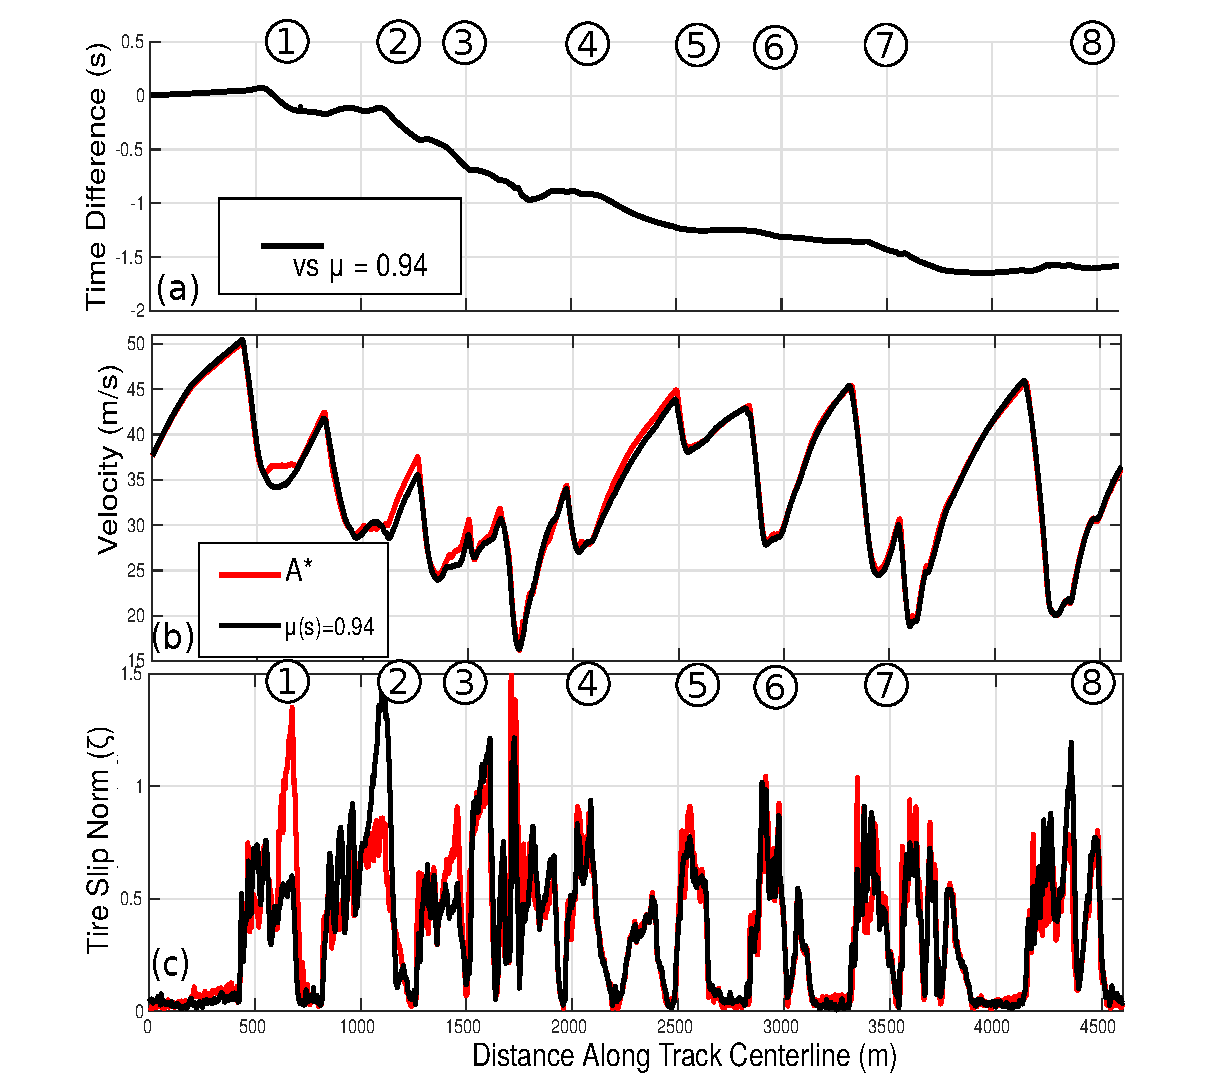
\includegraphics[width=3.4in]{figures/expAstarResults.eps}
\caption{Time difference between experimental dataset collected with A* result $\mu^*(s)$ and constant friction velocity profile at $\mu = 0.94$. Negative time distance corresponds to A* result being ahead. (b) Experimental velocities between both experimental datasets.
(c) Tire slip norm measurements for both datasets.}
\label{fig:muexpres}
\end{figure}  

 The experimental results show solid performance of the learned friction profile $\mu^\star(s)$. From Fig.~\ref{fig:muexpres}(a), the lap time using the learned friction profile is roughly 1.5 seconds faster than the lap time from the constant friction profile. A significant part of this improved performance comes through more efficient friction usage.
 For example, in sections \circled{2} and \circled{8}, learning to drive more cautiously enables the tire slip norm $\zeta$ to drop closer to 1, avoiding
 a costly understeer. In sections \circled{3} and \circled{7}, the A* algorithm has learned that more aggressive driving is possible, increasing $\zeta$ closer to 1.\footnote{Note that due to time constraints, both datasets were all taken on different dates, meaning some variation in weather and tire conditions is possible for each test.} 

\section{Conclusion}
This paper presents two complementary approaches to gradually improve the driving performance of an autonomous race car 
over time. Iterative learning control (ILC) formulations gradually determine the proper steering and throttle inputs to precisely track the desired racing trajectory. Experimental results at combined vehicle accelerations of 9 $\mathrm{m/s^2}$  indicate that the proposed algorithm can rapidly attenuate trajectory following errors over just two or three laps of racing. This paper also presents a trajectory modification algorithm to minimize experimental lap times by learning different acceleration limits for each turn on the track. An A* search algorithm is devised to search through experimental data and find the best value of $\mu$ for each portion of the track in order to globally minimize the resulting lap time. Key developments of this algorithm include designing an appropriate A* heuristic to minimize the needed computation time and designing the cost function to account for the physical difficulty of altering the vehicle's trajectory while understeering or oversteering.

\section*{Acknowledgment}

This research was supported by the National Science Foundation Graduate Research Fellowship Program (GRFP). The
authors would like to thank the members of the Dynamic
Design Lab at Stanford University and the Audi Electronics
Research Lab.

\bibliographystyle{IEEEtran}
\bibliography{Bibliography}


\end{document}
